\section{Tổng quan kết quả hiện thực}

Sau khi hoàn tất quá trình xây dựng và tích hợp các thành phần của hệ thống lên nền tảng Raspberry Pi 4, một loạt kiểm tra được thực hiện nhằm xác nhận cấu hình phần cứng và phần mềm đã đáp ứng đúng thiết kế. Kết quả tổng thể được trình bày thông qua các lệnh hệ thống, cho thấy môi trường Linux Embedded hoạt động ổn định với đầy đủ các thành phần nhân, thư viện và driver.

Về mặt hệ điều hành, Raspberry Pi 4 chạy bản phân phối nhúng được sinh ra từ Yocto Project. Cụ thể, nội dung tệp \texttt{/etc/os-release} cho thấy tên bản phân phối là \texttt{Poky (Yocto Project Reference Distro)} với phiên bản 5.0.11, mã nguồn Scarthgap, như được thể hiện trong Hình~\ref{fig:sys1}. Đây là phiên bản ổn định và tương đối mới của Yocto, cung cấp đầy đủ các lớp metadata cần thiết cho Raspberry Pi 4. Phiên bản nhân Linux được xác định qua lệnh \texttt{uname -a} là 6.6.63-v8, được biên dịch với chế độ \texttt{PREEMPT} để hỗ trợ thời gian thực, và chạy trên kiến trúc \texttt{aarch64} (64-bit).

\begin{figure}[H]
    \centering
    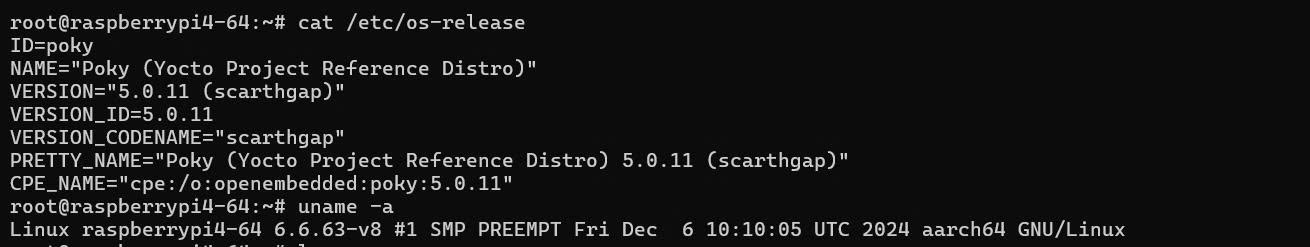
\includegraphics[width=0.9\linewidth]{image/sys1.jpg}
    \caption{Thông tin phiên bản hệ điều hành và nhân Linux}
    \label{fig:sys1}
\end{figure}

Thông tin chi tiết về CPU từ lệnh \texttt{lscpu} xác nhận bộ xử lý là ARM Cortex-A72 với 4 lõi, tốc độ tối đa 1500 MHz, mỗi lõi có 32KB L1d, 48KB L1i và chia sẻ 1MB L2 cache. Các cờ mở rộng như \texttt{fp}, \texttt{asimd}, \texttt{crc32}, \texttt{cpuid} cho biết hỗ trợ tính toán dấu phẩy động, SIMD và kiểm tra lỗi CRC. Đặc biệt, các lỗ hổng bảo mật phần cứng như Meltdown, Spectre v1 được giảm thiểu thông qua cơ chế làm sạch con trỏ người dùng, mặc dù Spectre v2 vẫn ở trạng thái dễ bị tấn công (Vulnerable) do đặc thù phần cứng ARM. Hình ảnh đầu ra của lệnh \texttt{lscpu} được trình bày trong Hình~\ref{fig:sys2}.

\begin{figure}[H]
    \centering
    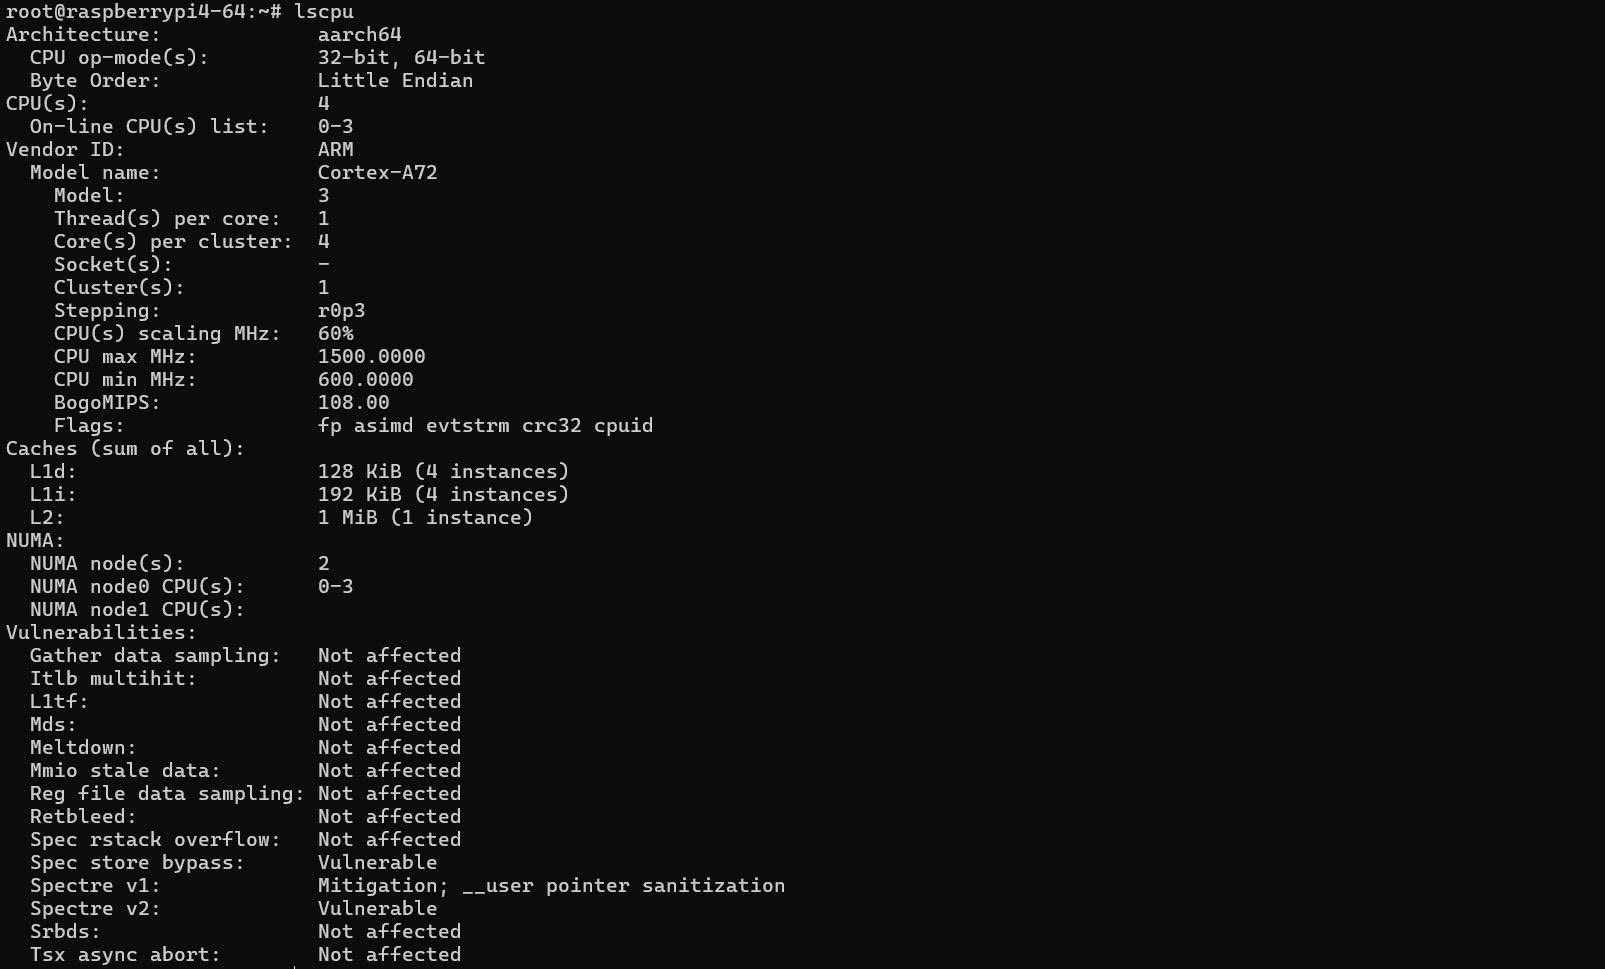
\includegraphics[width=0.9\linewidth]{image/sys2.jpg}
    \caption{Thông tin bộ xử lý và các lỗ hổng bảo mật}
    \label{fig:sys2}
\end{figure}

Dung lượng bộ nhớ RAM được kiểm tra qua lệnh \texttt{free -h} cho thấy tổng bộ nhớ vật lý là 8.008.064 KB (tương đương khoảng 7,8 GB), với phân vùng swap không được cấu hình. Lượng bộ nhớ đã sử dụng chỉ khoảng 115 MB trong khi bộ nhớ khả dụng lên tới 7,8 GB, chứng tỏ hệ thống nhúng có dư dả tài nguyên để chạy các ứng dụng giám sát và xử lý dữ liệu cảm biến. Mô hình phần cứng chính xác được đọc từ tệp \texttt{/proc/device-tree/model} là Raspberry Pi 4 Model B Rev 1.5, một trong những phiên bản phổ biến cho phát triển ứng dụng IoT biên. Cuối cùng, thông điệp chào mừng từ \texttt{/etc/issue} nhắc lại bản phân phối Poky 5.0.11, khẳng định một lần nữa môi trường Yocto đã được khởi tạo thành công. Toàn bộ các thông số về bộ nhớ, mô hình board và phiên bản phân phối được tổng hợp trong Hình~\ref{fig:sys3}.

\begin{figure}[H]
    \centering
    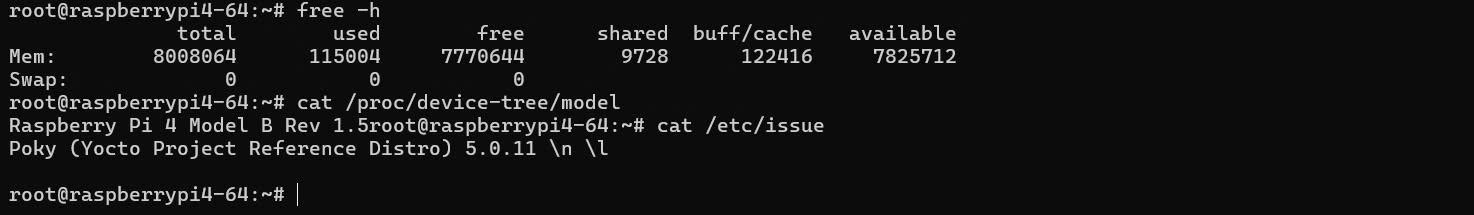
\includegraphics[width=0.9\linewidth]{image/sys3.jpg}
    \caption{Dung lượng bộ nhớ và thông tin board Raspberry Pi 4}
    \label{fig:sys3}
\end{figure}

Như vậy, các kết quả kiểm tra ban đầu cho thấy nền tảng Linux Embedded được xây dựng đúng theo thiết kế, với đầy đủ khả năng về hiệu năng, bộ nhớ và hỗ trợ phần cứng, sẵn sàng cho các bước tích hợp driver RS485, giao diện người dùng và các dịch vụ IoT. Toàn bộ các thông số này đóng vai trò là cơ sở để đánh giá hoạt động ổn định của hệ thống trong các phần tiếp theo.

\section{Bảo mật hệ thống}
\subsection{Selinux}
Nhóm thực hiện đã tích hợp thành công cơ chế bảo mật SELinux vào hệ thống nhúng xây dựng trên nền tảng Yocto Linux nhằm tăng cường khả năng kiểm soát truy cập và bảo vệ hệ thống trước các hành vi truy cập trái phép. SELinux được cấu hình hoạt động ở chế độ \texttt{enforcing} với policy \texttt{targeted}, cho phép áp dụng các chính sách bảo mật bắt buộc (Mandatory Access Control - MAC) lên các tiến trình và tài nguyên quan trọng của hệ thống.

Trong quá trình hiện thực, nhóm đã bổ sung layer \texttt{meta-selinux} vào môi trường build Yocto để tích hợp các thành phần cần thiết như SELinux userspace, policy package và các công cụ quản lý security context. Sau khi build và khởi động hệ thống, trạng thái SELinux được kiểm tra bằng lệnh \texttt{sestatus}. Kết quả cho thấy SELinux đã được kích hoạt thành công với các thông số:
\begin{itemize}
\item SELinux status: \texttt{enabled}
\item Current mode: \texttt{enforcing}
\item Loaded policy name: \texttt{targeted}
\end{itemize}

Policy \texttt{targeted} là chế độ phổ biến của SELinux, trong đó chỉ các tiến trình và dịch vụ quan trọng được áp dụng chính sách kiểm soát truy cập nghiêm ngặt, giúp giảm ảnh hưởng đến hoạt động thông thường của hệ thống đồng thời vẫn đảm bảo mức độ bảo mật cao. Khi hệ thống hoạt động, SELinux tự động kiểm tra quyền truy cập giữa các tiến trình và tài nguyên thông qua security context. Nếu một tiến trình cố gắng thực hiện hành động không được policy cho phép, hệ thống sẽ ghi nhận và từ chối thao tác đó.

Hình~\ref{fig:selinux-enforcing} cho thấy các bản ghi audit được tạo ra khi SELinux phát hiện hành vi truy cập không hợp lệ. Các thông báo \texttt{avc: denied} chứng minh rằng cơ chế MAC của SELinux đang hoạt động và thực hiện chặn truy cập trái phép đến các thiết bị hoặc tài nguyên hệ thống. Điều này giúp hạn chế nguy cơ leo thang đặc quyền, sửa đổi trái phép dữ liệu hệ thống và tăng cường khả năng bảo vệ firmware trong môi trường nhúng công nghiệp.

\begin{figure}[H]
    \centering
    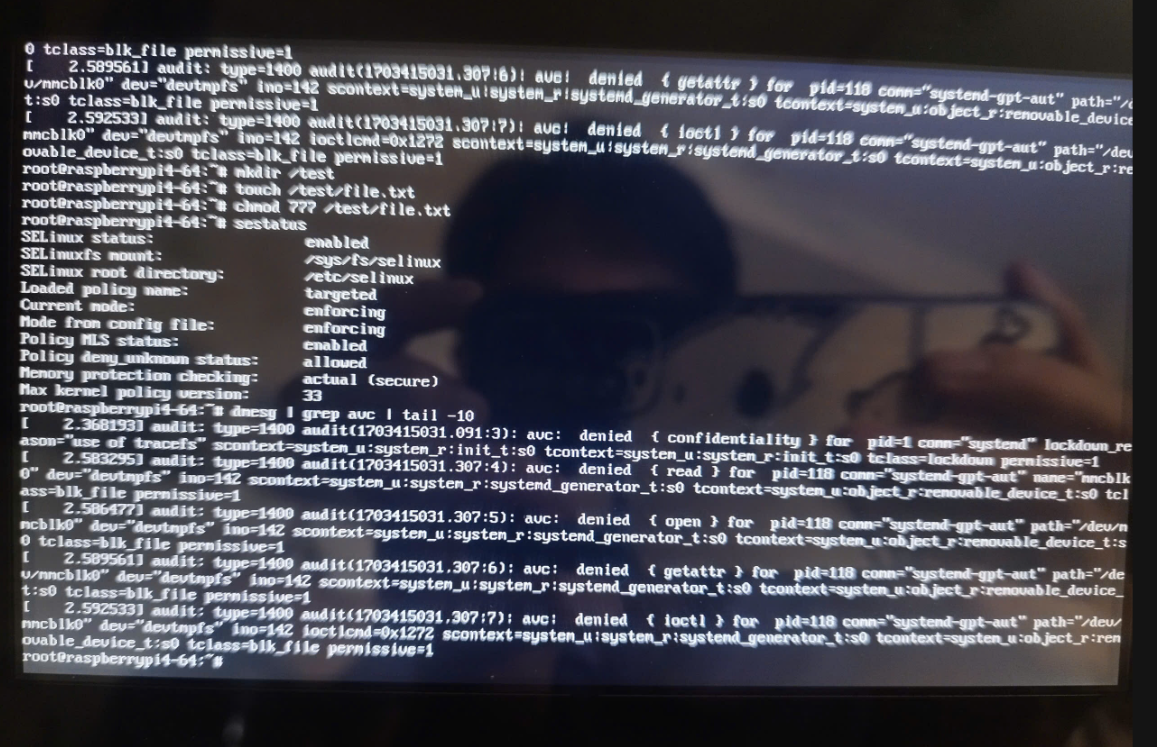
\includegraphics[width=0.7\linewidth]{image/selinux1.png}
    \caption{SELinux hoạt động ở chế độ enforcing với policy targeted}
    \label{fig:selinux-enforcing}
\end{figure}

\subsection{dm-verity}
Kết quả thực nghiệm cho thấy hệ thống đã khởi động thành công với root filesystem được bảo vệ bởi cơ chế \texttt{dm-verity}. Root filesystem được mount ở chế độ chỉ đọc thông qua thiết bị \texttt{/dev/mapper/vroot}, đảm bảo mọi block dữ liệu đều được kiểm tra tính toàn vẹn trước khi sử dụng. Sau khi boot hoàn tất, hệ thống vẫn hoạt động ổn định, hỗ trợ kết nối mạng và thực thi các thao tác quản trị cơ bản. Việc tích hợp \texttt{dm-verity} giúp phát hiện và ngăn chặn các hành vi chỉnh sửa trái phép firmware, từ đó nâng cao độ tin cậy và mức độ bảo mật cho hệ thống nhúng trong môi trường công nghiệp và IoT.

\begin{figure}[H]
    \centering
    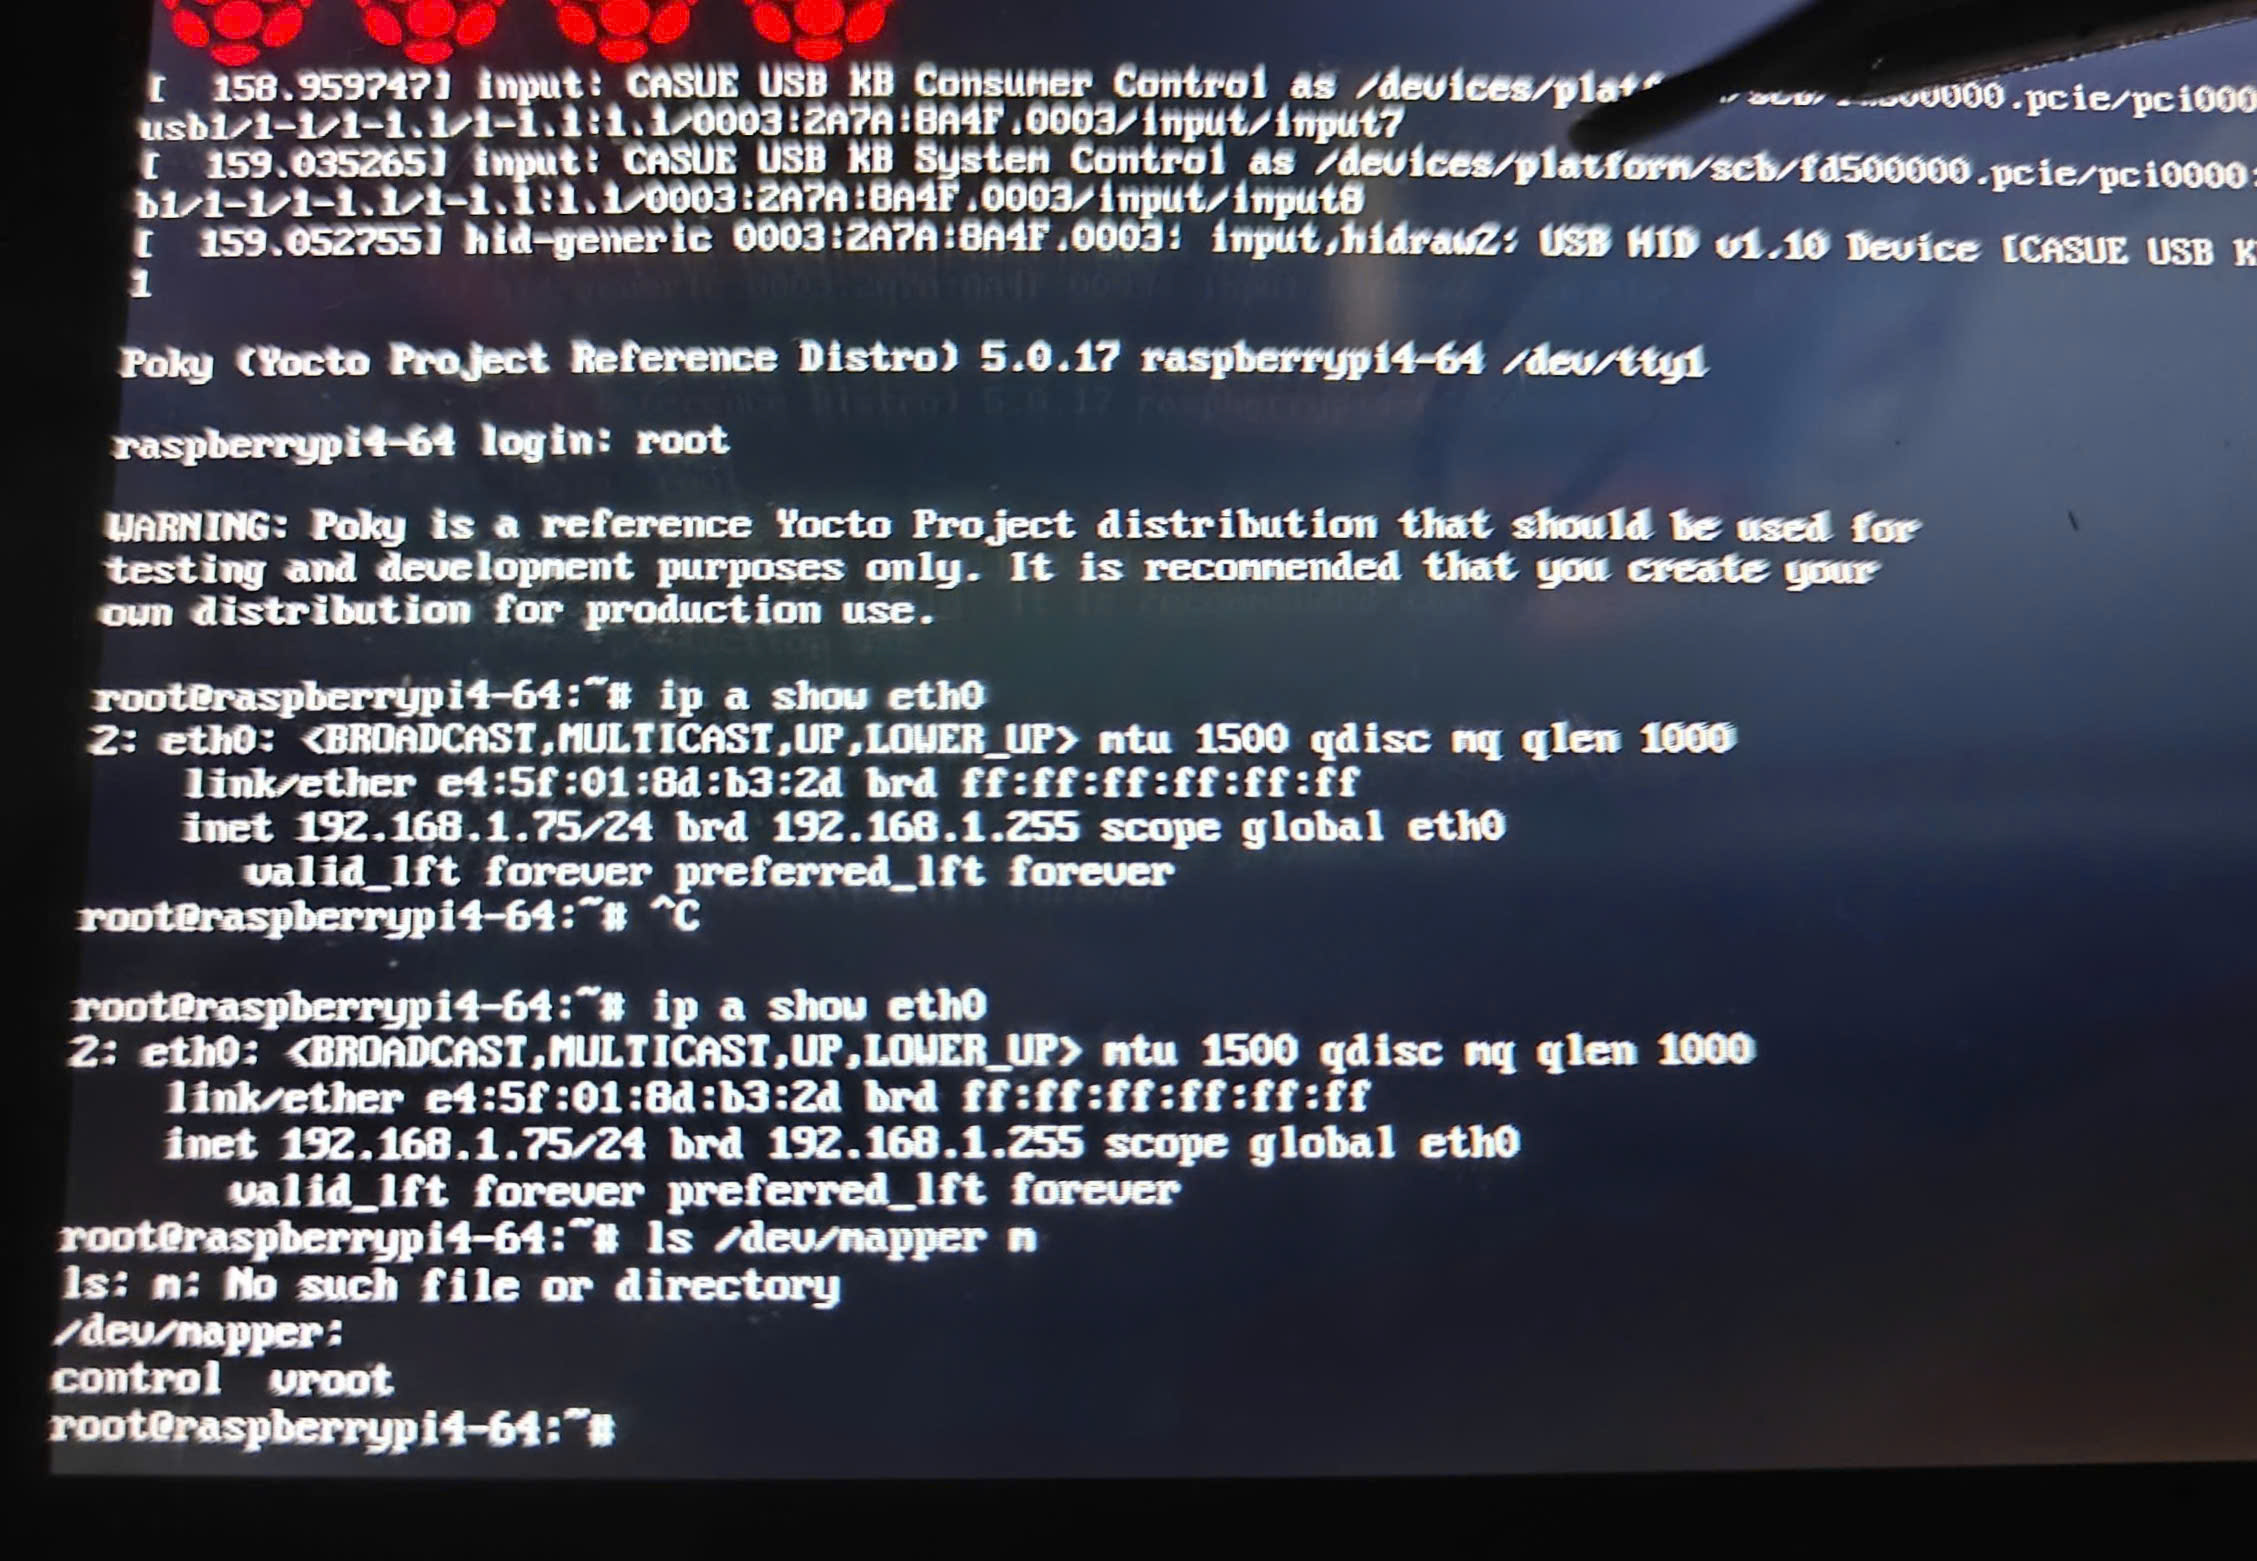
\includegraphics[width=0.7\linewidth]{image/dmverity1.jpg}
    \caption{Hệ thống khởi động thành công với root filesystem được bảo vệ bởi dm-verity}
    \label{fig:dmverity-boot}
\end{figure}

\section{Device Driver}
\subsection{Driver I2C}

\begin{figure}[H]
    \centering
    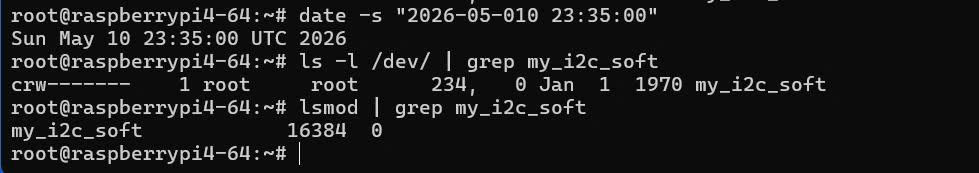
\includegraphics[width=0.8\linewidth]{image/testi2c.jpg}
    \caption{Tính khả dụng của Driver}
    \label{fig:warning_block}
\end{figure}

Kết quả thực nghiệm cho thấy kernel module \texttt{my\_i2c\_soft} đã được nạp thành công vào Linux Kernel. Điều này được xác nhận thông qua lệnh \texttt{lsmod}, trong đó module xuất hiện trong danh sách các kernel module đang hoạt động của hệ thống.

Bên cạnh đó, hệ thống cũng đã tạo thành công device file \texttt{/dev/my\_i2c\_soft} với kiểu thiết bị ký tự (character device), thể hiện qua ký tự \texttt{c} ở đầu kết quả của lệnh \texttt{ls -l}. Device file này đóng vai trò là giao diện giao tiếp giữa user space và kernel space, cho phép các ứng dụng người dùng truy cập tới driver thông qua các system call như \texttt{open()}, \texttt{read()}, \texttt{write()} và \texttt{ioctl()}.

Sự xuất hiện đồng thời của kernel module trong danh sách module đang hoạt động và device file trong thư mục \texttt{/dev} cho thấy driver đã được khởi tạo đúng cách, đăng ký thành công với Linux Kernel và sẵn sàng phục vụ quá trình giao tiếp với phần cứng I2C Software.

Sau khi hoàn tất quá trình tích hợp driver và cơ chế giao tiếp I2C Software, hệ thống tiếp tục được kiểm thử bằng cách hiện thực chương trình hiển thị dữ liệu cảm biến lên màn hình OLED SSD1306. Chương trình thực hiện đọc dữ liệu từ các cảm biến môi trường và cập nhật trực tiếp lên màn hình OLED thông qua giao tiếp I2C, bao gồm các thông số như nhiệt độ, độ ẩm và trạng thái hoạt động của hệ thống.

\begin{figure}[H]
    \centering
    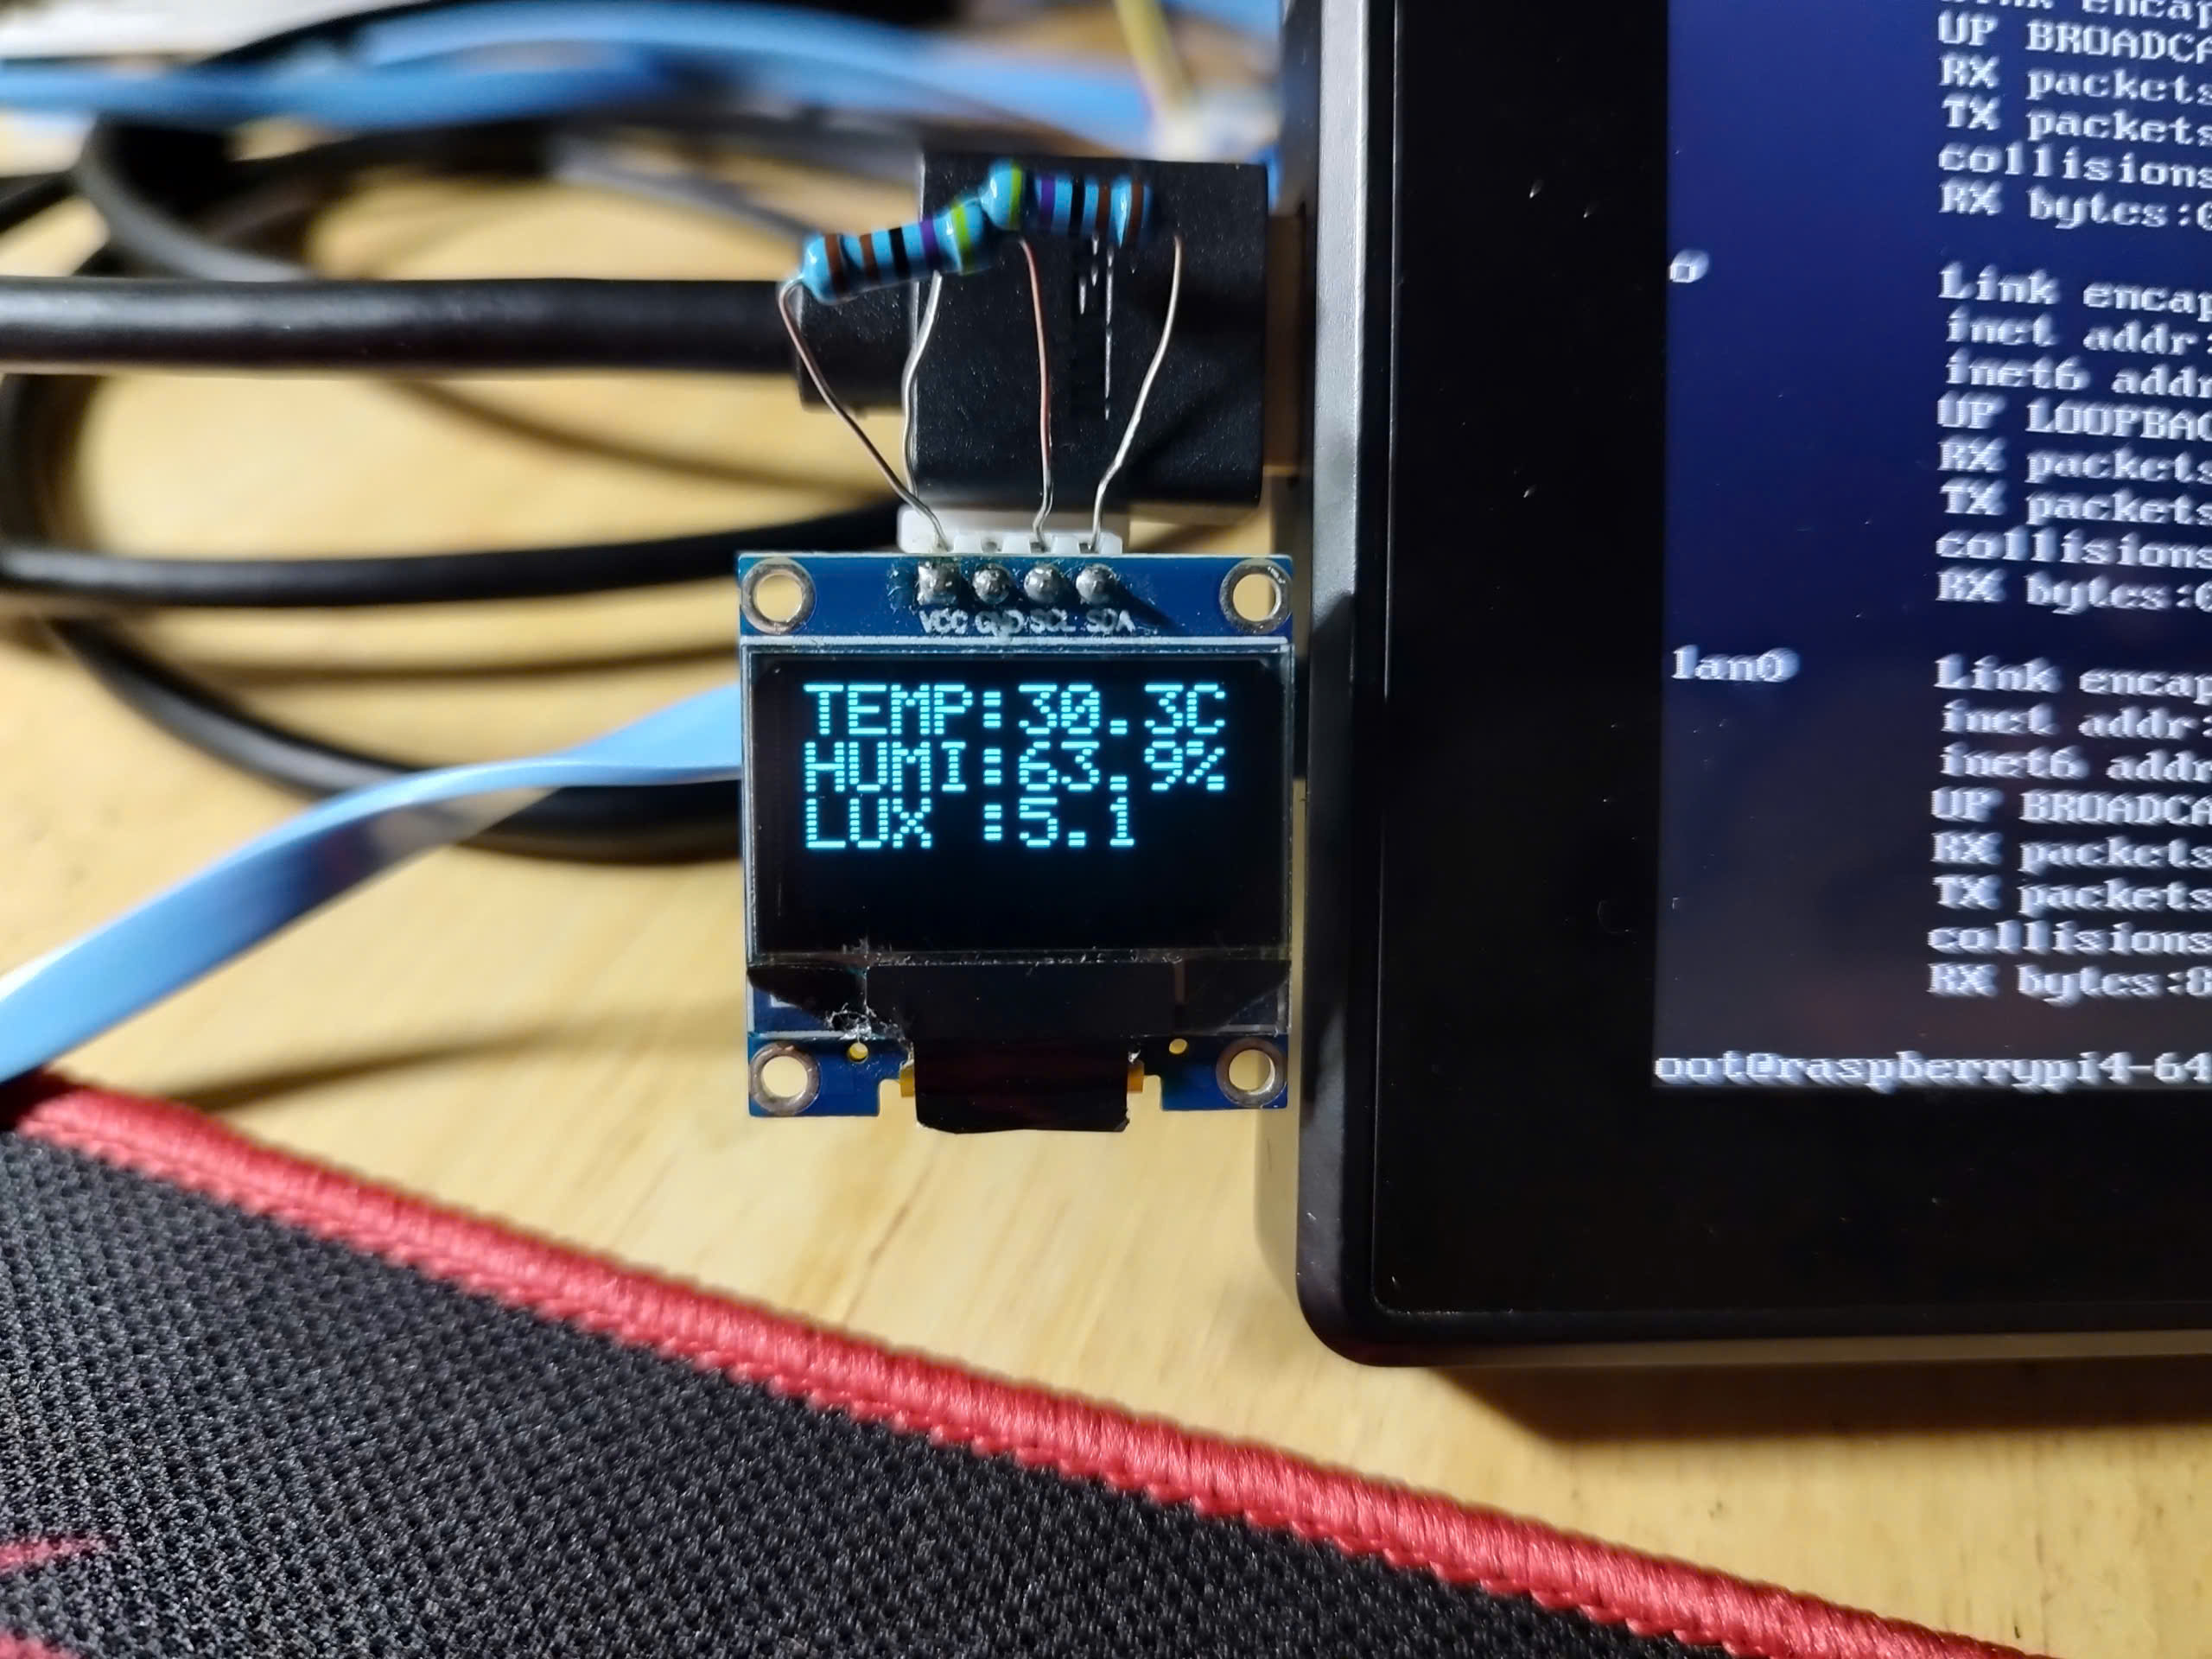
\includegraphics[width=0.7\linewidth]{image/oled.jpg}
    \caption{Kết quả hiển thị dữ liệu cảm biến trên màn hình OLED SSD1306}
    \label{fig:oled_result}
\end{figure}

Kết quả này cho thấy driver I2C đã hoạt động đúng chức năng, đồng thời xác nhận khả năng giao tiếp ổn định giữa hệ điều hành Linux nhúng và các thiết bị ngoại vi thông qua cơ chế Linux Device Driver. Việc hiển thị thành công dữ liệu cảm biến trên màn hình OLED cũng là cơ sở để tiếp tục phát triển các chức năng giám sát và cảnh báo trực quan trong hệ thống nhúng phục vụ các ứng dụng công nghiệp và IoT.

\subsection{Driver RS485 Modbus RTU}
Sau khi hoàn tất quá trình build và tích hợp vào hệ thống Yocto, driver được kiểm thử trên Raspberry Pi 4 với hệ điều hành Linux Embedded xây dựng từ Yocto Project để đảm bảo rằng kernel module đã được nạp thành công vào Linux Kernel và device file được tạo chính xác trong thư mục \texttt{/dev}.

\begin{figure}[H]
    \centering
    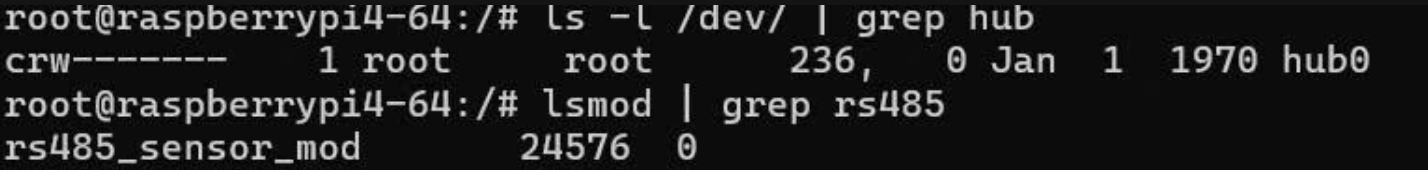
\includegraphics[width=0.95\linewidth]{image/rs485gd2.png}
    \caption{Tính khả dụng của Driver}
    \label{fig:warning_block}
\end{figure}

Kết quả trên cho thấy Character Device đã được tạo thành công và kernel module đang hoạt động trong hệ thống. Điều này xác nhận quá trình khởi tạo driver, đăng ký Character Device và cơ chế autoload module đã được triển khai chính xác trong môi trường Linux Embedded.

Driver tiếp tục được kiểm thử thông qua quá trình đọc dữ liệu cảm biến từ thiết bị RS485. Các giá trị nhiệt độ, độ ẩm, áp suất và PM2.5 được cập nhật ổn định theo chu kỳ polling.

\begin{figure}[H]
    \centering
    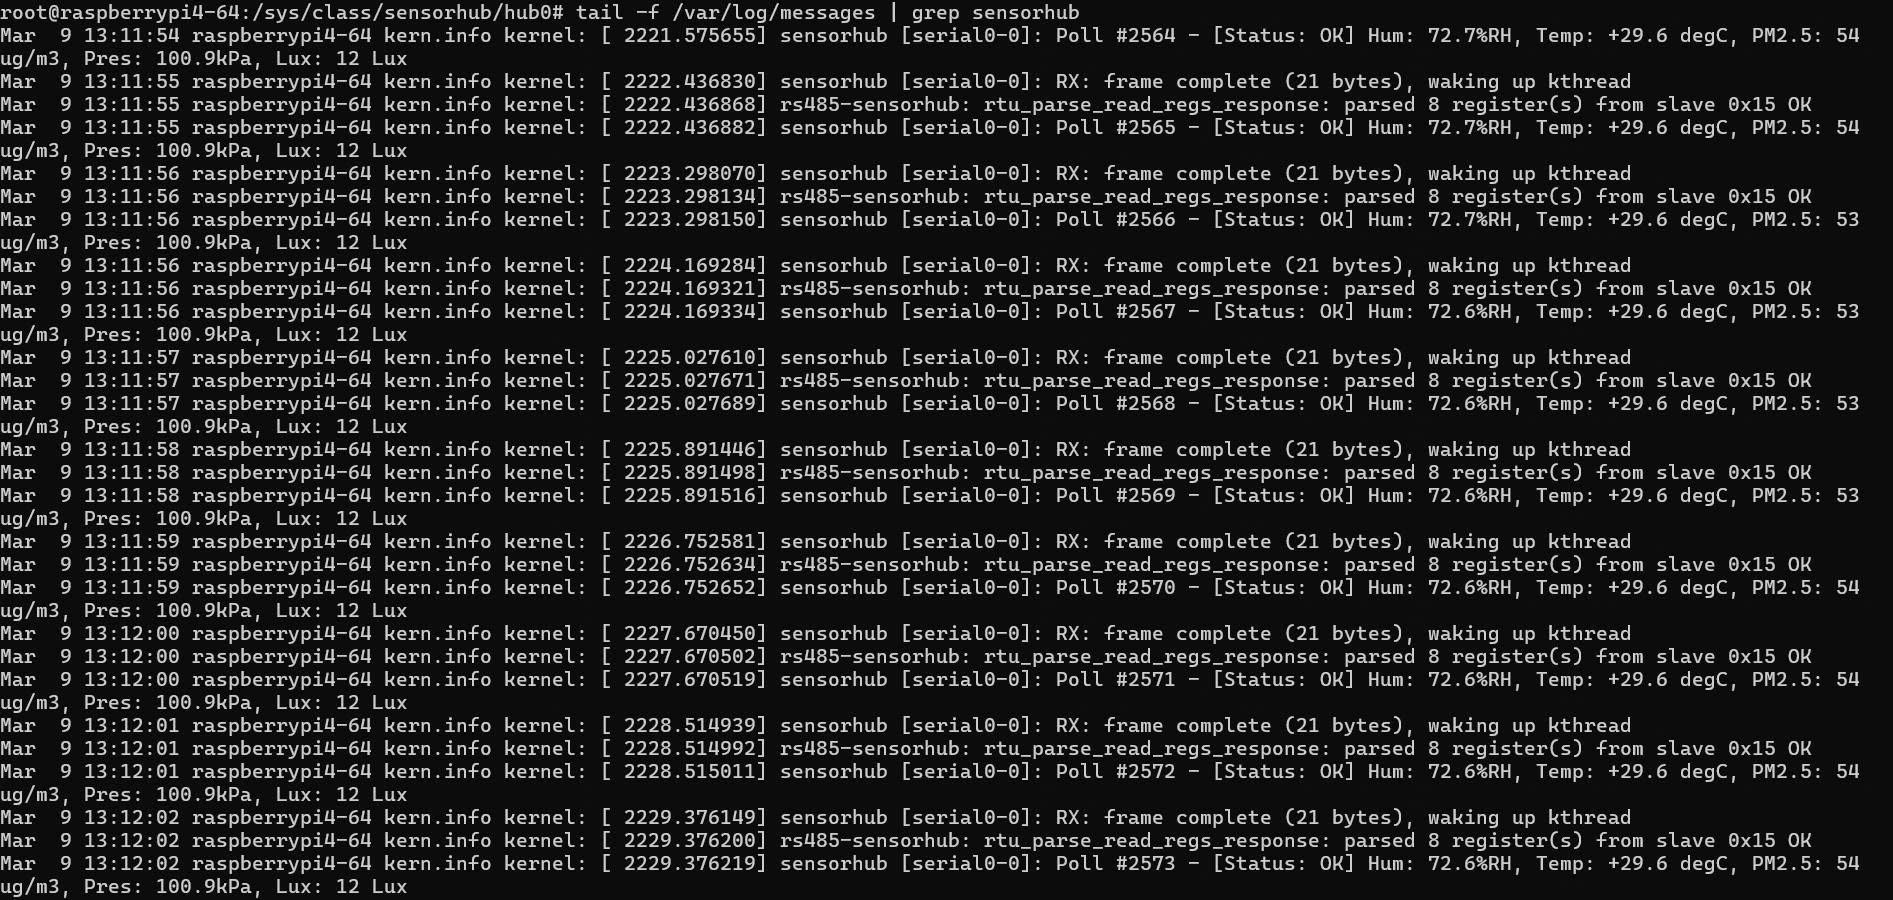
\includegraphics[width=1\linewidth]{image/datars485.jpg}
    \caption{Thu thập dữ liệu từ Driver}
    \label{fig:warning_block}
\end{figure}

Đồng thời dữ liệu có thể được truy cập từ User Space thông qua device file do driver tạo ra, đóng vai trò như một giao diện trung gian giữa ứng dụng người dùng và Kernel Space. Thông qua cơ chế Character Device, các tiến trình ở User Space có thể thực hiện các thao tác chuẩn như đọc dữ liệu cảm biến mà không cần truy cập trực tiếp vào phần cứng hoặc tham gia vào các cơ chế xử lý phức tạp trong kernel.

\begin{figure}[H]
    \centering
    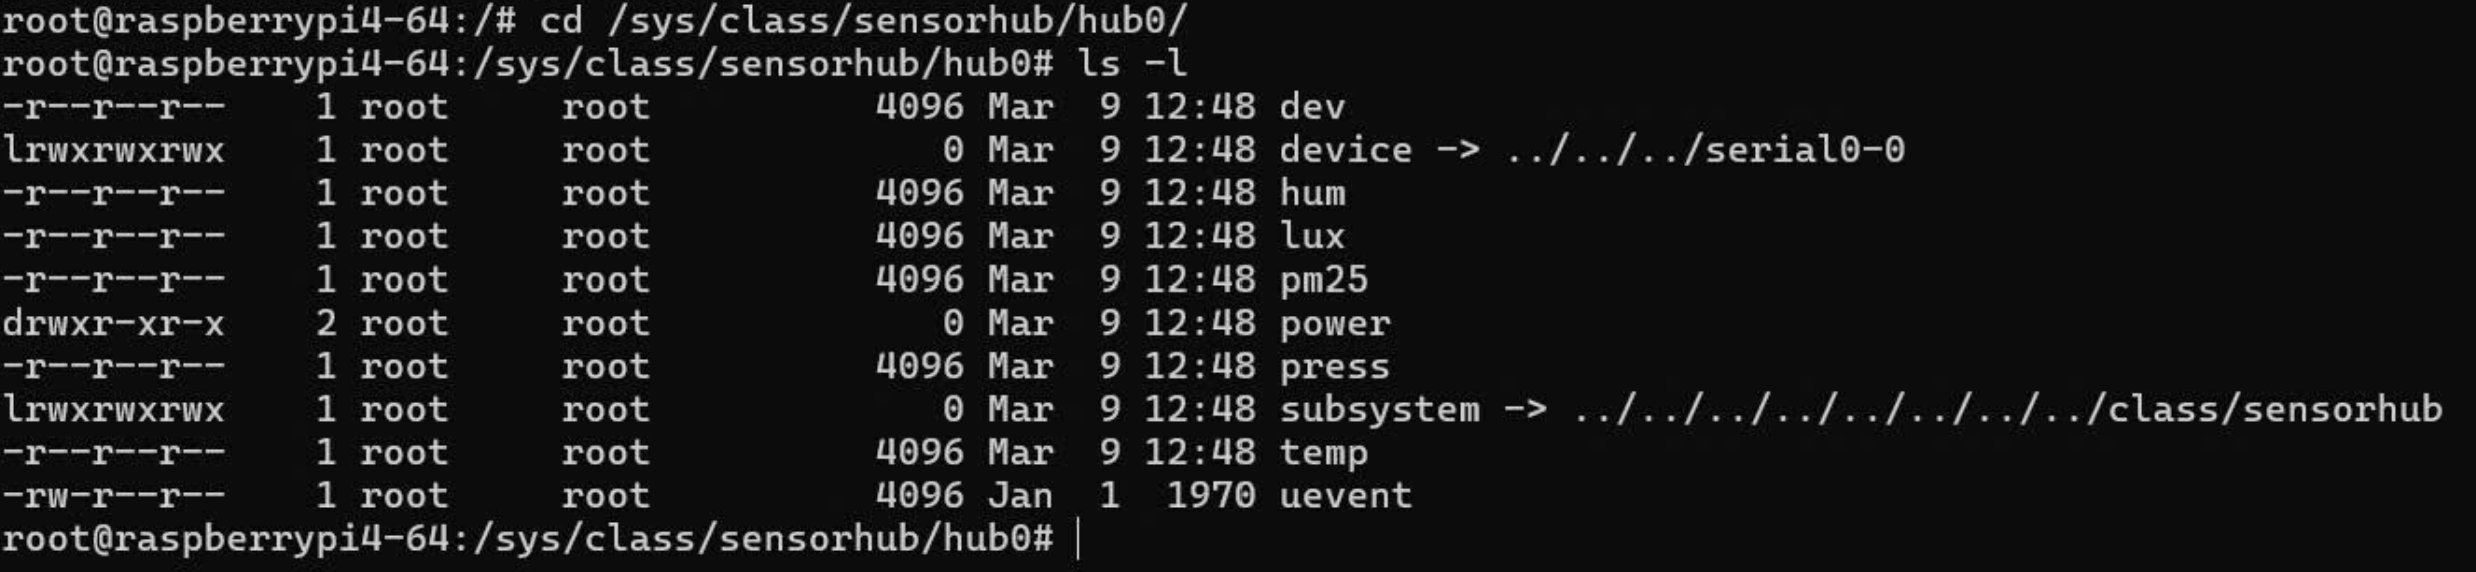
\includegraphics[width=0.95\linewidth]{image/drv_file.png}
    \caption{Lưu trữ dữ liệu từ Driver}
    \label{fig:warning_block}
\end{figure}
Sau khi chuyển thư mục vào \texttt{/sys/class/sensorhub/hub0/}, ta liệt kê các tệp trong sysfs của driver. Kết quả hiển thị lần lượt các tệp như \texttt{dev}, \texttt{num}, \texttt{lux}, \texttt{pm25}, \texttt{press}, \texttt{temp} cùng các liên kết tượng trưng \texttt{device} và \texttt{subsystem}. Sự xuất hiện của các tệp \texttt{lux}, \texttt{pm25}, \texttt{press}, \texttt{temp} cho thấy driver đã cung cấp giao diện sysfs để đọc dữ liệu cảm biến, cho phép ứng dụng ở không gian người dùng truy xuất trực tiếp các giá trị cường độ ánh sáng, nồng độ bụi mịn, áp suất và nhiệt độ. Như vậy, toàn bộ các thành chính của driver bao gồm Character Device, kernel module và sysfs interface đều hoạt động đúng như thiết kế.
Kết quả thực nghiệm cho thấy driver hoạt động ổn định trên nền tảng Raspberry Pi 4, đáp ứng yêu cầu truyền nhận dữ liệu Modbus RTU trong môi trường Linux Embedded sử dụng Yocto Project.

\section{Khối xử lý AI}
Sau giai đoạn thiết lập cấu hình và thực thi huấn luyện, khối xử lý AI đã đạt được các kết quả thực nghiệm quan trọng. Phần này trình bày chi tiết về các sản phẩm đầu ra của mô hình, các thông số kỹ thuật và đánh giá sơ bộ về khả năng dự báo dựa trên các nhật ký thực thi thực tế.

\subsection{Các tệp tin sản phẩm sau hiện thực (Artifacts)}

Quá trình hiện thực hóa hai chương trình \texttt{main.py} và \texttt{convert.py} đã tạo ra một bộ sản phẩm mô hình hoàn chỉnh, sẵn sàng để triển khai lên lớp Gateway bảo mật.
    \begin{figure}[H]
    \centering
    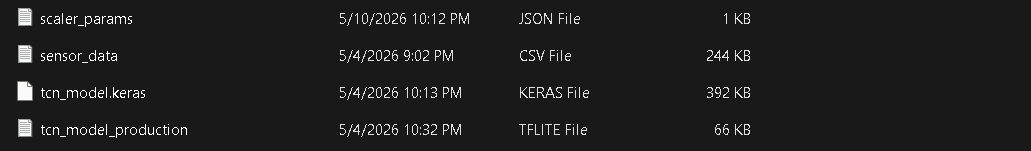
\includegraphics[width=0.9\textwidth]{image/file_ketqua.png}
    \caption{cấu trúc file sau khi train mô hình}
    \label{fig:meta-ota}
  \end{figure}
\begin{itemize}
    \item \textbf{Mô hình huấn luyện (\texttt{tcn\_model.keras}):} 
    Tệp tin này lưu trữ toàn bộ kiến trúc mạng TCN cùng các trọng số đã được tối ưu hóa trong quá trình huấn luyện ở định dạng số thực 32-bit (FP32). Dung lượng lưu trữ của mô hình trên đĩa là khoảng 392 KB.

    \item \textbf{Mô hình tối ưu (\texttt{tcn\_model\_production.tflite}):} 
    Đây là kết quả của quá trình chuyển đổi sang định dạng TensorFlow Lite kết hợp kỹ thuật định lượng hóa Float16 (Float16 Quantization). Kích thước tệp chỉ còn khoảng 66 KB, giảm gần 6 lần so với mô hình gốc, giúp giảm đáng kể yêu cầu bộ nhớ và tăng tốc độ suy luận trên thiết bị nhúng.

    \item \textbf{Tệp tham số chuẩn hóa (\texttt{scaler\_params.json}):} 
    Tệp JSON này lưu trữ các giá trị cực tiểu và cực đại (\texttt{min}, \texttt{max}) của 7 đặc trưng môi trường được sử dụng trong quá trình huấn luyện. Việc lưu lại các tham số này đảm bảo dữ liệu đầu vào tại thời điểm triển khai thực tế sẽ được chuẩn hóa hoàn toàn nhất quán với dữ liệu đã dùng để huấn luyện mô hình.
\end{itemize}

\subsection{Đặc tính kỹ thuật và Tài nguyên hệ thống}

Mô hình TCN được hiện thực với kiến trúc tối ưu nhằm cân bằng giữa độ chính xác dự báo và mức tiêu thụ tài nguyên phần cứng của thiết bị Raspberry Pi 4.

\begin{table}[H]
\centering
\caption{Thông số kỹ thuật của mô hình TCN sau huấn luyện}
\label{tab:tcn-technical-specs}
\begin{tabular}{|p{7cm}|p{4cm}|}
\hline
\textbf{Thông số} & \textbf{Giá trị hiện thực} \\
\hline
Tổng số tham số (Total Params) & 23{,}233 \\
\hline
Dung lượng tham số trong RAM & 90.75 KB \\
\hline
Kích thước tệp thực thi (\texttt{.tflite}) & 66 KB \\
\hline
Độ trễ suy luận mỗi bước (Latency per step) & 6 -- 7 ms \\
\hline
\end{tabular}
\end{table}

Việc mô hình chỉ chiếm khoảng 90.75 KB trong bộ nhớ RAM là một kết quả thực nghiệm rất khả quan. Điều này cho thấy mô hình có thể hoạt động song song với các dịch vụ nền quan trọng như SELinux, dịch vụ xác minh toàn vẹn hệ thống (\textit{dm-verity}) và các tác vụ giám sát bảo mật khác mà không gây ra hiện tượng tràn bộ nhớ hay ảnh hưởng đến độ ổn định của hệ thống.

\subsection{Phân tích quá trình huấn luyện và hội tụ}

Quá trình huấn luyện thực tế trên tập dữ liệu gồm 2000 mẫu đã cho thấy kiến trúc TCN có khả năng học tập ổn định và hội tụ tốt.

\begin{itemize}
    \item \textbf{Cơ chế Early Stopping:} 

    Hệ thống đã hiện thực thành công cơ chế giám sát tự động với tham số \texttt{patience = 15}. Theo nhật ký thực thi, quá trình huấn luyện tự động dừng tại epoch thứ 297 khi hàm mất mát trên tập kiểm định không còn được cải thiện đáng kể. Kết quả này cho thấy mô hình đã đạt đến trạng thái bão hòa về sai số. Việc dừng huấn luyện đúng thời điểm giúp hạn chế hiện tượng quá khớp (\textit{overfitting}) và tránh lãng phí tài nguyên tính toán.

    \begin{figure}[H]
    \centering
    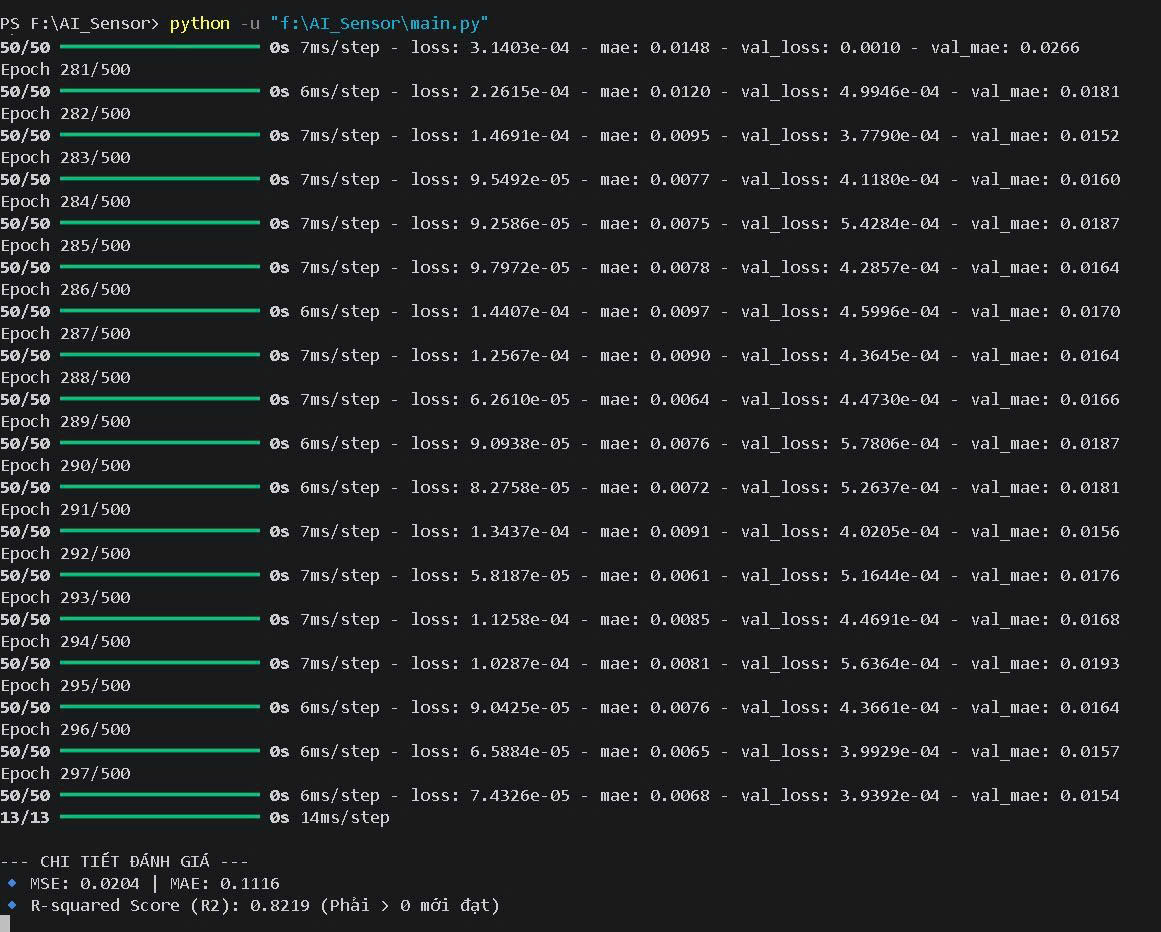
\includegraphics[width=0.9\textwidth]{image/ketqua_train.jpg}
    \caption{Kết quả train mô hình}
    \label{fig:Train-AI}

  \end{figure}
    \item \textbf{Đường cong tổn thất (Loss Curve):}

    Quan sát biểu đồ tổn thất trong Hình~\ref{fig:training-loss-curve}, giá trị \textit{Train Loss} và \textit{Validation Loss} giảm mạnh trong các epoch đầu tiên và dần ổn định ở mức tiệm cận gần bằng 0 sau khoảng 50 epoch. Khoảng cách rất nhỏ giữa hai đường cong trong suốt quá trình huấn luyện cho thấy mô hình có tính ổn định cao, không xuất hiện dấu hiệu phân kỳ, đồng thời duy trì khả năng tổng quát hóa tốt trên dữ liệu chưa từng được quan sát.

    \begin{figure}[H]
    \centering
    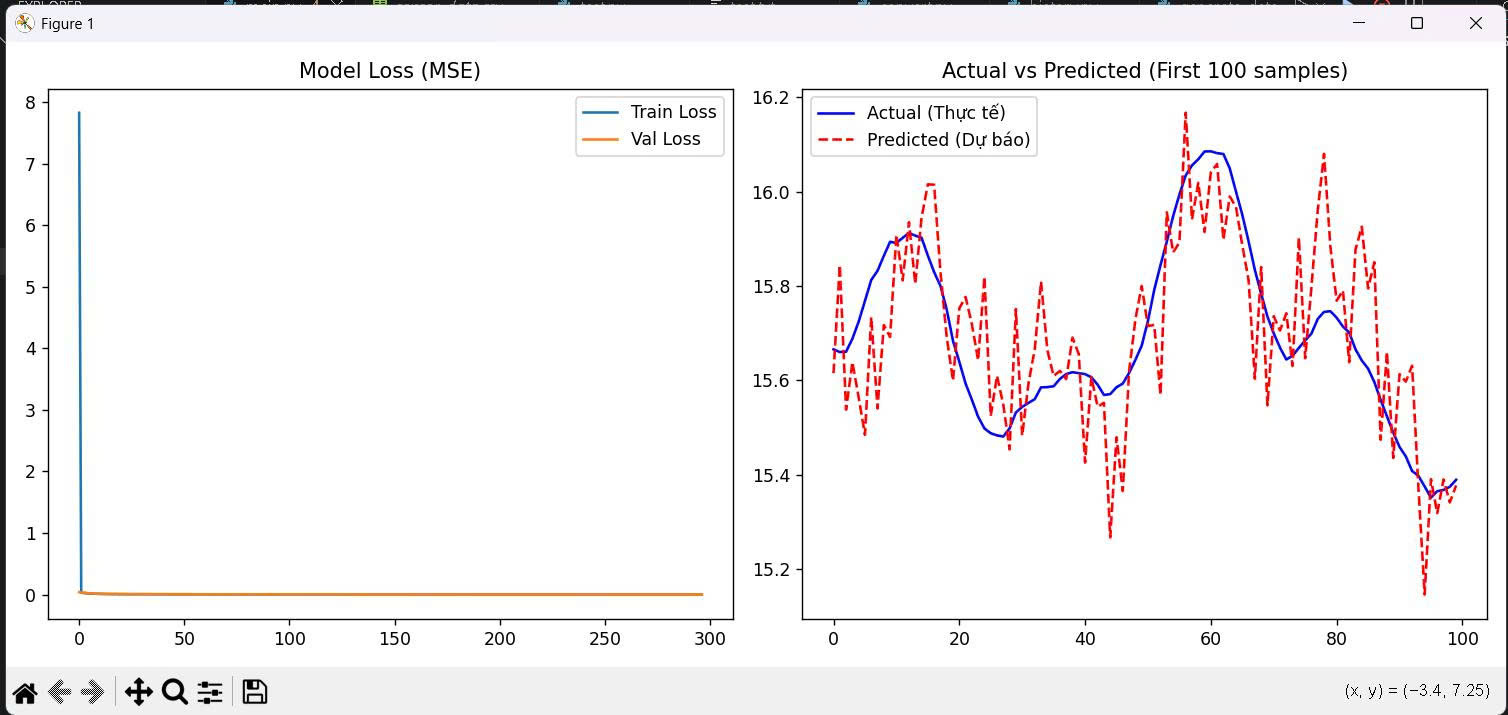
\includegraphics[width=0.6\textwidth]{image/dothi.jpg}
    \caption{Đồ thị train mô hình}
    \label{fig:training-loss-curve}
     \end{figure}

\end{itemize}
\subsection{Đánh giá sơ bộ các chỉ số sai số (Metrics)}

Dựa trên kết quả thực thi của hàm \texttt{evaluate\_model()}, hệ thống đã tự động tính toán các chỉ số đánh giá định lượng trên tập dữ liệu kiểm thử. Các chỉ số này phản ánh mức độ sai lệch giữa giá trị dự báo của mô hình và giá trị đo thực tế, đồng thời cung cấp cơ sở để đánh giá chất lượng của mô hình trước khi triển khai lên thiết bị biên.

\begin{itemize}
    \item \textbf{Sai số bình phương trung bình (Mean Squared Error -- MSE):} đạt giá trị \textbf{0.0204}.

    Chỉ số MSE được xác định theo công thức:

    \begin{equation}
        \mathrm{MSE}
        =
        \frac{1}{n}
        \sum_{i=1}^{n}
        \left(y_i - \hat{y}_i\right)^2
        =
        0.0204
    \end{equation}

    Giá trị MSE nhỏ cho thấy độ lệch bình phương trung bình giữa giá trị dự đoán và giá trị thực tế là rất thấp. Điều này chứng minh mô hình TCN có khả năng mô phỏng chính xác xu hướng biến động của nồng độ bụi mịn PM2.5.

    \item \textbf{Sai số tuyệt đối trung bình (Mean Absolute Error -- MAE):} đạt giá trị \textbf{0.1116}.

    Chỉ số này biểu thị độ sai lệch tuyệt đối trung bình giữa dự đoán và thực tế. Với giá trị chỉ khoảng 0.11 đơn vị, có thể thấy mỗi dự báo của mô hình chỉ chênh lệch rất nhỏ so với dữ liệu đo thực tế, phù hợp với yêu cầu của các hệ thống giám sát môi trường thời gian thực.

    \item \textbf{Hệ số xác định (\(R^2\) Score):} đạt giá trị \textbf{0.8219}.

    Hệ số \(R^2\) phản ánh mức độ mà mô hình giải thích được biến thiên của dữ liệu đầu ra. Giá trị 0.8219 cho thấy mô hình giải thích được khoảng 82.19\% sự biến thiên của nồng độ PM2.5 dựa trên các đặc trưng đầu vào như nhiệt độ, độ ẩm, áp suất khí quyển và các thông số môi trường khác. Đây là một kết quả rất tích cực đối với một mô hình gọn nhẹ được tối ưu cho hệ thống nhúng.
\end{itemize}

Bên cạnh các chỉ số định lượng, Hình~\ref{fig:training-loss-curve} còn cung cấp đánh giá trực quan về quá trình huấn luyện và chất lượng dự báo của mô hình.

\begin{itemize}
    \item \textbf{Biểu đồ Loss Curve (bên trái):} 

    Giá trị \textit{Train Loss} giảm rất nhanh từ mức ban đầu khoảng 7.8 xuống gần 0 chỉ sau vài epoch đầu tiên. Đồng thời, đường \textit{Validation Loss} cũng bám sát đường huấn luyện trong toàn bộ quá trình, cho thấy mô hình hội tụ ổn định và không xuất hiện hiện tượng quá khớp rõ rệt.

    \item \textbf{Biểu đồ Actual vs Predicted (bên phải):}

    Đường dự báo (nét đứt màu đỏ) bám sát đường dữ liệu thực tế (đường xanh liên tục) trong hầu hết các thời điểm. Mô hình tái hiện chính xác xu hướng tăng giảm của tín hiệu PM2.5, kể cả tại các vùng có biến động nhanh. Sai lệch nhỏ giữa hai đường chủ yếu xuất hiện tại các đỉnh cực trị, điều này là đặc trưng thường gặp trong các bài toán dự báo chuỗi thời gian.
\end{itemize}

Tổng hợp các kết quả trên cho thấy mô hình TCN không chỉ đạt chất lượng dự báo tốt về mặt định lượng mà còn thể hiện khả năng tổng quát hóa ổn định trên dữ liệu chưa từng xuất hiện trong quá trình huấn luyện. Với kích thước nhỏ gọn, tốc độ suy luận nhanh và độ chính xác cao, mô hình hoàn toàn đáp ứng yêu cầu triển khai trên hệ thống Secure Edge AI sử dụng Raspberry Pi 4.

\subsection{Kiểm định khả năng Inference trên phần cứng Raspberry Pi 4}

Sau khi hoàn tất quy trình triển khai, hệ thống được đưa vào kiểm định thực tế nhằm đánh giá hai yếu tố sống còn của một hệ thống nhúng: Độ nhạy đáp ứng (\textit{Accuracy response}) và Tốc độ suy luận (\textit{Inference speed}).

\subsubsection{Đánh giá độ nhạy dự đoán qua thực nghiệm tác động môi trường}

Trong kịch bản này, nhóm thực hiện tác động trực tiếp bằng nguồn khói vật lý để quan sát khả năng phản hồi của mô hình AI. Nhật ký hệ thống ghi nhận sự tương quan chặt chẽ giữa giá trị cảm biến đo được và giá trị AI dự đoán:

    \begin{figure}[H]
    \centering
    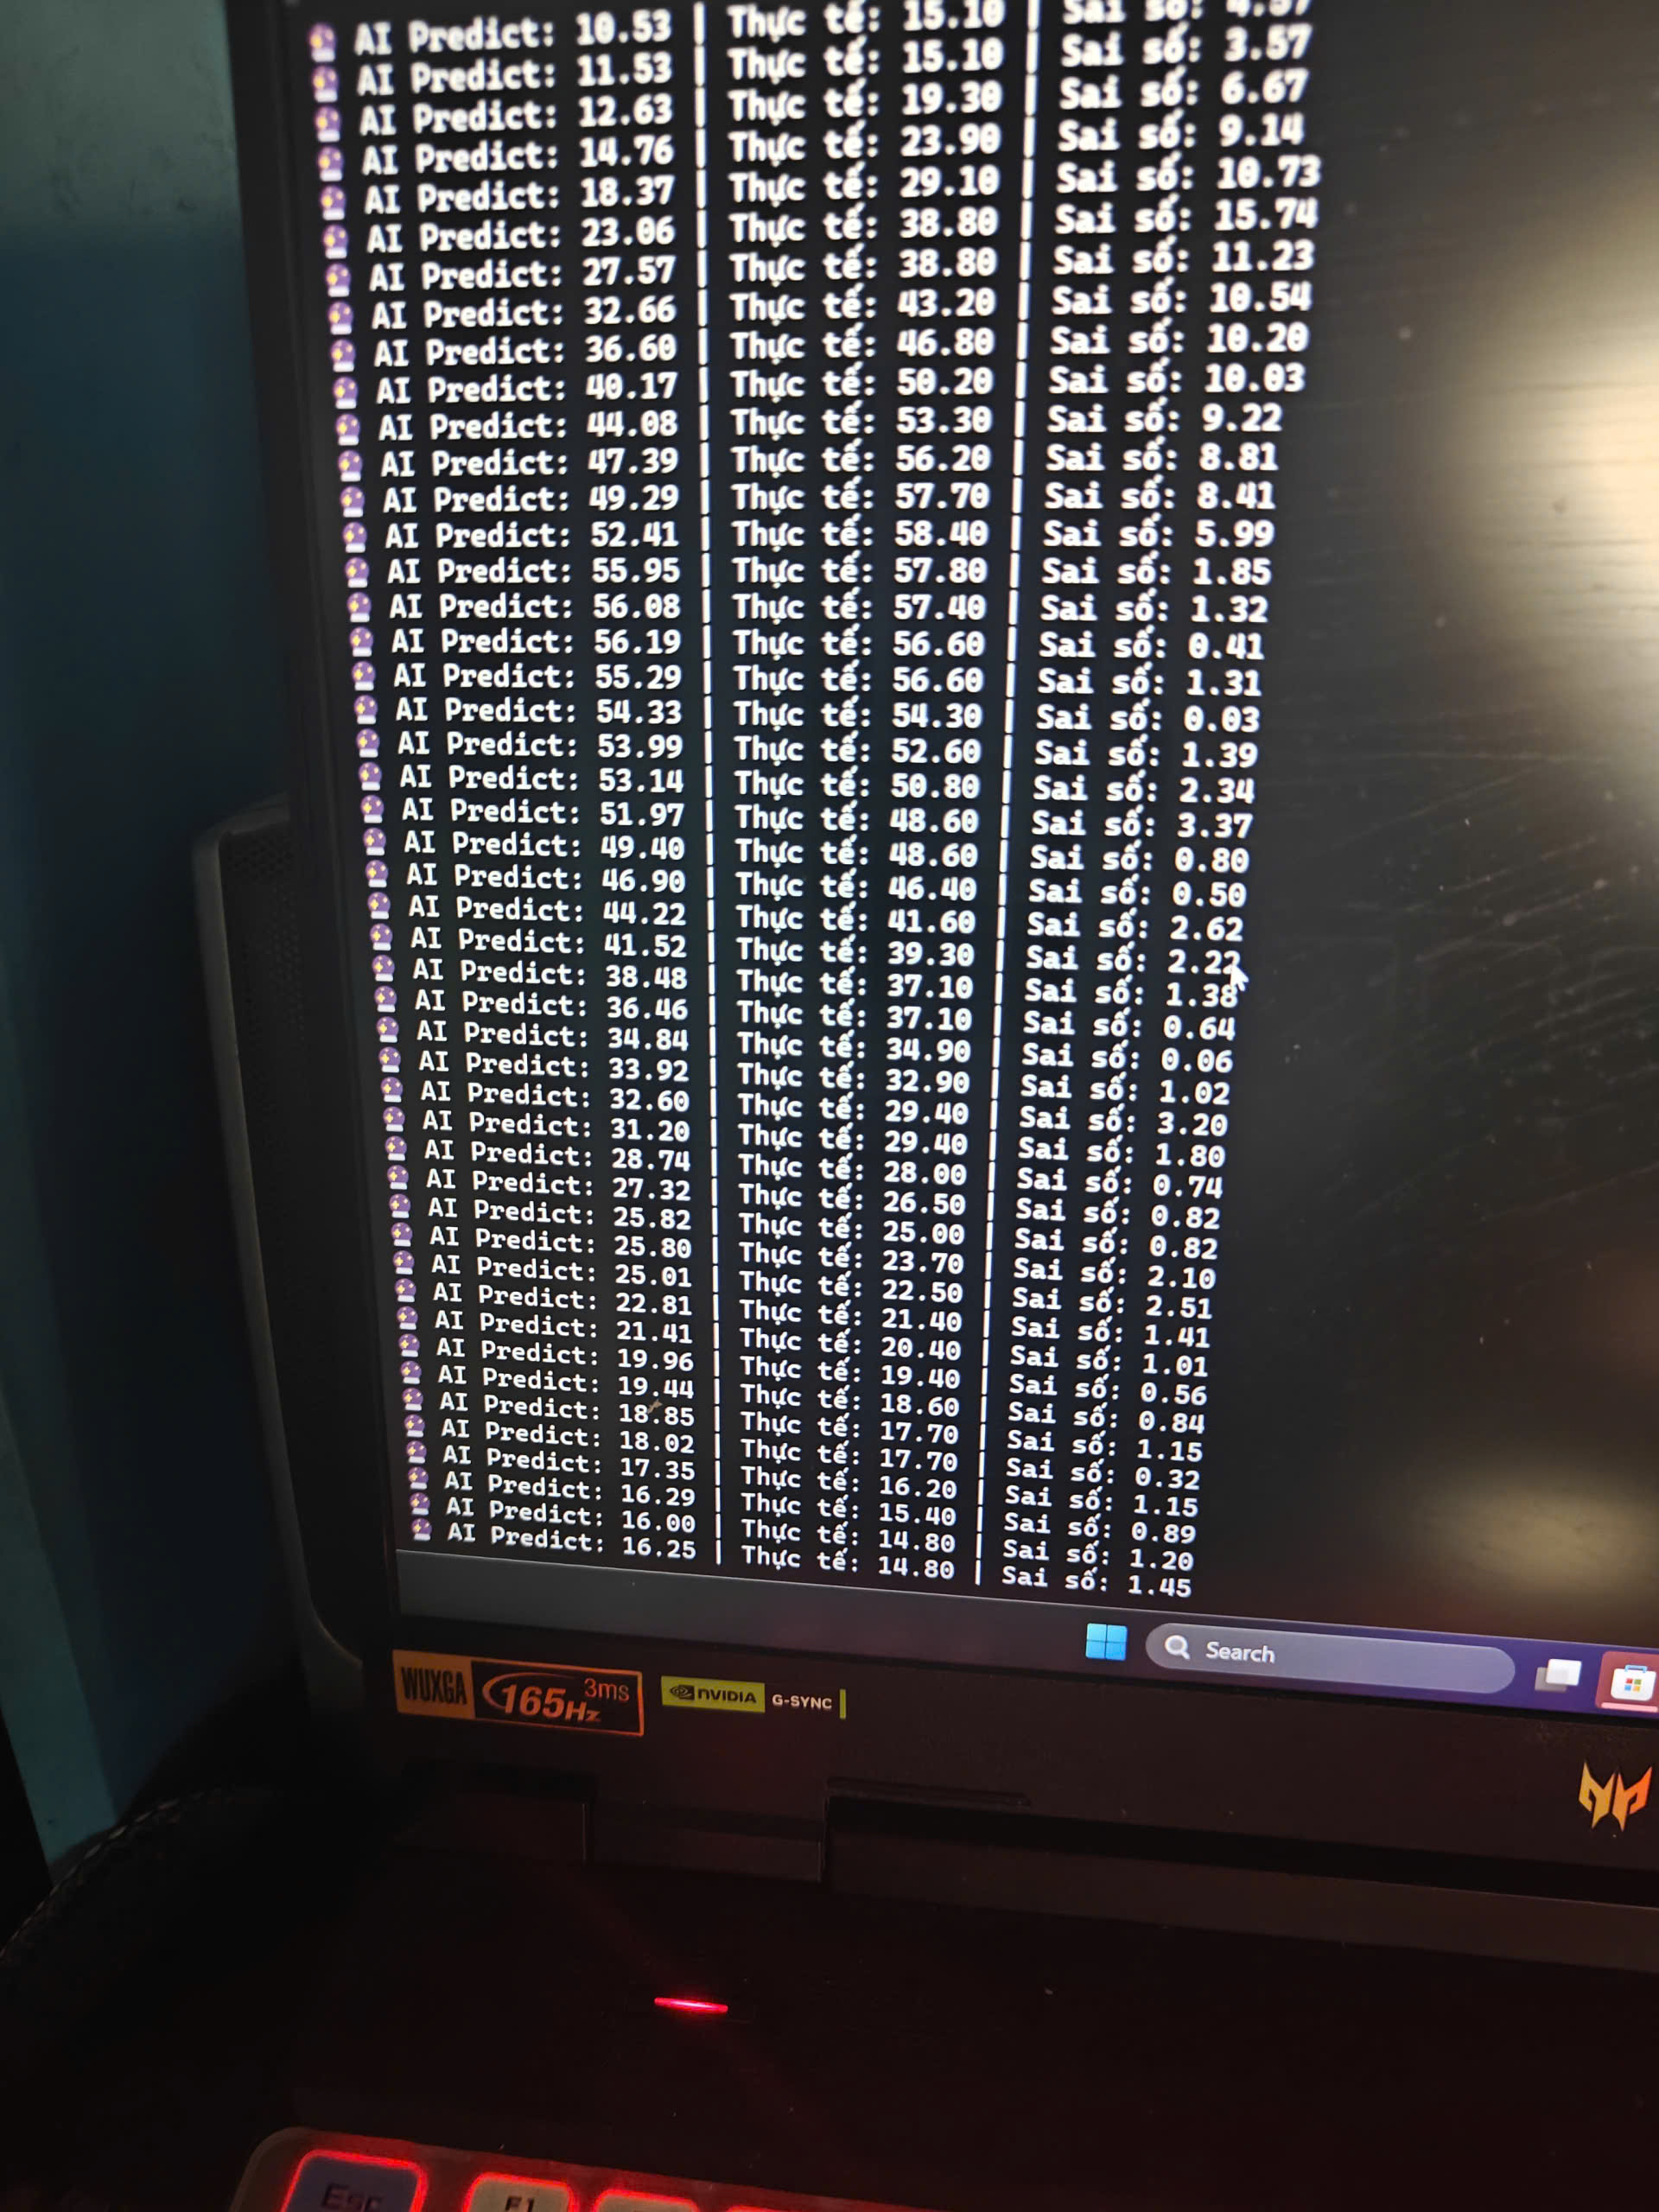
\includegraphics[width=0.5\textwidth]{image/fire.jpg}
    \caption{Kết quả test}
    \label{fig:ketqua-test}
     \end{figure}

\begin{itemize}
    \item \textbf{Phân tích biến thiên:} Khi nồng độ khói tăng mạnh từ 15.10 lên mức đỉnh 58.40, mô hình AI ngay lập tức phản hồi với giá trị dự đoán tăng tương ứng từ 10.53 lên 52.41.

    \item \textbf{Sai số tuyệt đối:} Qua bảng số liệu (Hình x), sai số trung bình duy trì ở mức thấp (dao động từ 0.32 đến 2.51 trong điều kiện ổn định). Điều này chứng minh mô hình không bị nhiễu bởi các yếu tố môi trường ngoài ý muốn và có độ tin cậy cao trong việc nhận diện nồng độ khói đậm đặc.

    \item \textbf{Khả năng hồi quy:} Khi khói tan, AI Predict giảm mượt mà về mức 16.25, bám sát giá trị thực tế 14.80, cho thấy thuật toán có tính ổn định cao và không xảy ra hiện tượng tràn số hay treo logic khi dữ liệu đầu vào biến động lớn.
\end{itemize}

\subsubsection{Đánh giá hiệu năng thời gian thực (Inference Time)}

Hiệu năng tính toán là yếu tố then chốt để hệ thống có thể đưa ra cảnh báo kịp thời. Qua nhật ký thực thi chi tiết trên phần cứng Pi 4 (Hình y), các thông số đo được như sau:

    \begin{figure}[H]
    \centering
    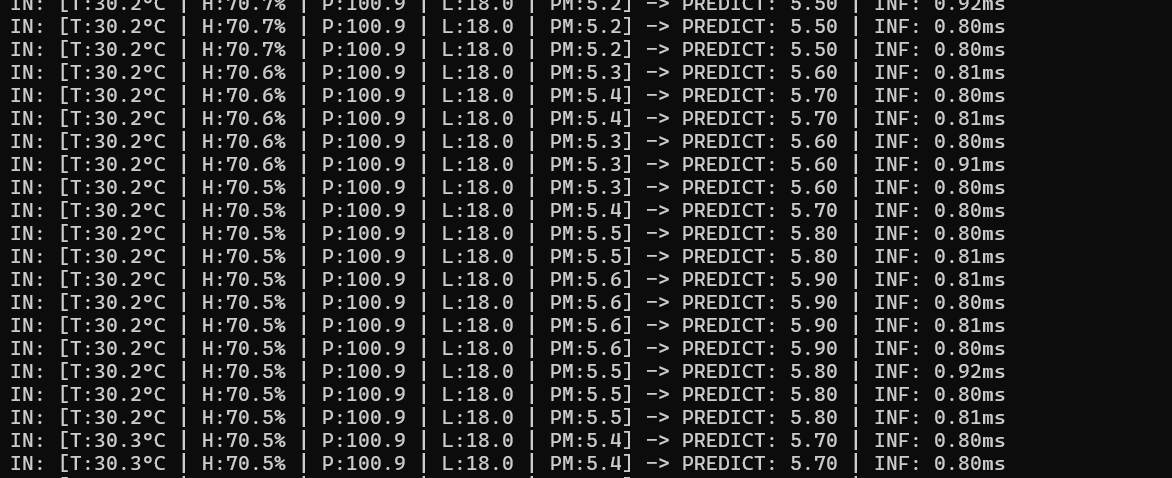
\includegraphics[width=0.9\textwidth]{image/infers.png}
    \caption{Kết quả Inference}
    \label{fig:ketqua-test}
     \end{figure}

\begin{itemize}
    \item \textbf{Thời gian suy luận (Inference Time - INF):} Hệ thống đạt tốc độ xử lý cực nhanh, trung bình chỉ mất từ 0.80ms đến 0.92ms cho mỗi lần suy luận.

    \item \textbf{Nhận xét:} Với thời gian dưới 1ms, đây là một kết quả cực kỳ ấn tượng đối với phần cứng nhúng như Raspberry Pi 4. Điều này cho phép CPU dành tài nguyên cho các tác vụ khác như duy trì kết nối mạng, xử lý giao diện Web và sẵn sàng cho các tiến trình cập nhật OTA mà không gây trễ hệ thống.

    \item \textbf{Sự ổn định của luồng dữ liệu:} Các chỉ số đầu vào (Nhiệt độ $\sim$30.2$^\circ$C, Độ ẩm $\sim$70.5\%, Áp suất $\sim$100.9) được xử lý song song với quá trình dự đoán PREDICT mà không làm biến động thời gian INF. Sự ổn định này khẳng định rằng mô hình đã được tối ưu hóa tốt về mặt cấu trúc (mạng nơ-ron thu gọn hoặc lượng tử hóa), phù hợp hoàn hảo cho các ứng dụng giám sát thời gian thực.
\end{itemize}

\subsubsection{Tổng kết khả năng thực thi}

Việc kết hợp giữa độ chính xác cao (sai số thấp khi đốt khói) và tốc độ suy luận siêu việt (dưới 1ms) đã khẳng định sự thành công trong việc hiện thực hóa mô hình AI lên thiết bị nhúng. Hệ thống hoàn toàn đáp ứng được các kịch bản cứu hộ, cảnh báo sớm và sẵn sàng phối hợp cùng khối OTA để cập nhật các bộ tham số tối ưu hơn trong tương lai mà không làm gián đoạn vận hành.

\section{Công cụ Secure-Yocto Builder}

\subsection{Kết quả hiện thực công cụ Secure-Yocto Builder}

Sau quá trình phát triển, công cụ Secure-Yocto Builder đã được hoàn thiện với giao diện Web TUI (\textit{Terminal User Interface}) trực quan, chạy trên nền tảng Flask và tích hợp đầy đủ các tính năng cấu hình hệ thống từ xa.

\subsubsection{Giao diện cấu hình thiết bị mục tiêu (Target Device)}

Hệ thống cho phép người dùng lựa chọn giữa phần cứng thực tế (Raspberry Pi 4-64) và môi trường giả lập (QEMU x86-64). Khi người dùng thay đổi tùy chọn, hệ thống sẽ thực hiện cập nhật biến \texttt{MACHINE} trong tệp \texttt{local.conf} ngay lập tức.

\begin{figure}[H]
    \centering
    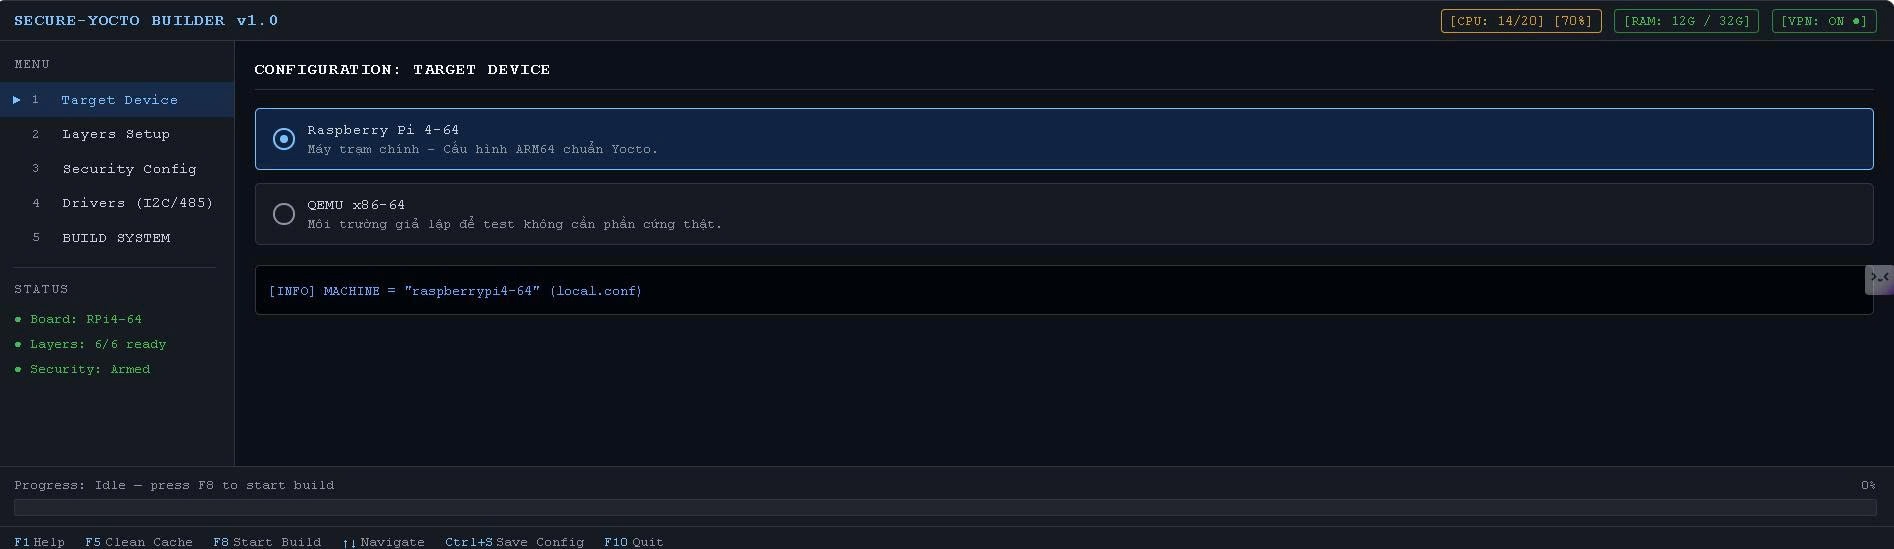
\includegraphics[width=0.85\textwidth]{image/image_be4279.jpg}
    \caption{Giao diện lựa chọn Target Device và phản hồi cập nhật \texttt{local.conf}.}
    \label{fig:target-device-ui}
\end{figure}

\subsubsection{Quản lý lớp (Layer Setup) và Recipe bổ sung}

Tính năng này cho phép người dùng theo dõi trạng thái các lớp (\textit{Layers}) hiện có và thêm mới các gói phần mềm (\textit{Packages}) vào bản build. Hệ thống có cơ chế kiểm tra sự tồn tại của Recipe trong metadata trước khi thực hiện chèn lệnh \texttt{IMAGE\_INSTALL:append}.

\begin{itemize}
    \item \textbf{Trường hợp thành công:} Khi người dùng nhập tên gói hợp lệ (ví dụ: \texttt{htop}), hệ thống thông báo xác nhận đã chèn thành công.
    \item \textbf{Trường hợp lỗi:} Nếu tên gói không tồn tại, hệ thống sẽ báo lỗi \texttt{[ERROR]} để ngăn chặn việc build thất bại do thiếu Recipe.
\end{itemize}

\begin{figure}[H]
    \centering
    \begin{minipage}{0.48\textwidth}
        \centering
        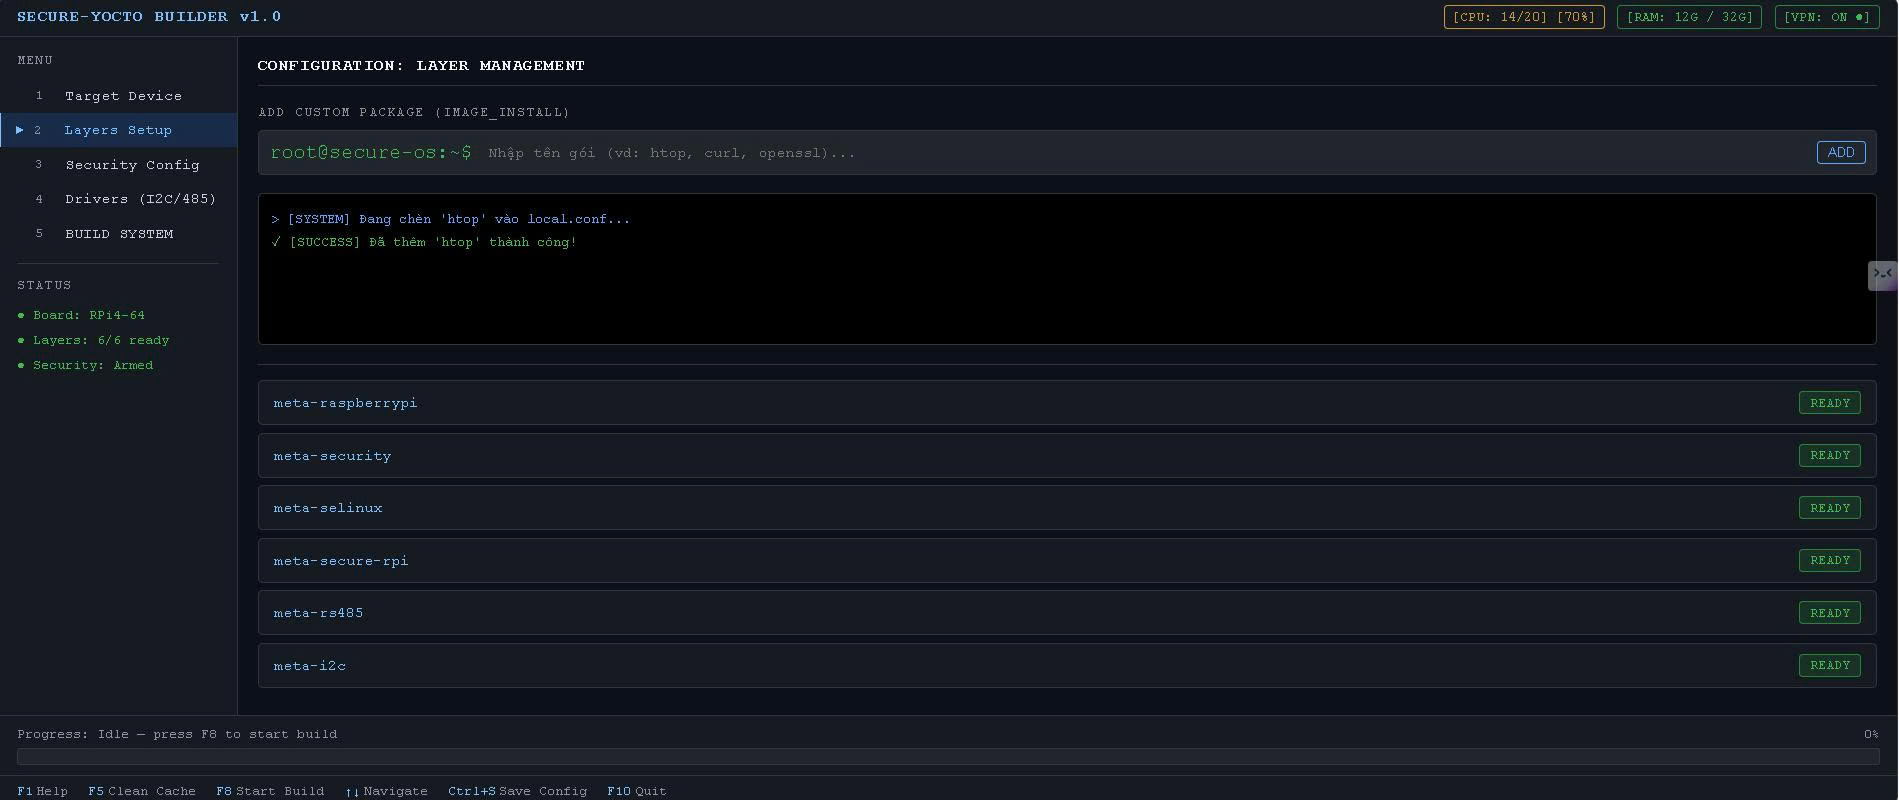
\includegraphics[width=\textwidth]{image/image_be4275.jpg}
    \end{minipage}
    \hfill
    \begin{minipage}{0.48\textwidth}
        \centering
        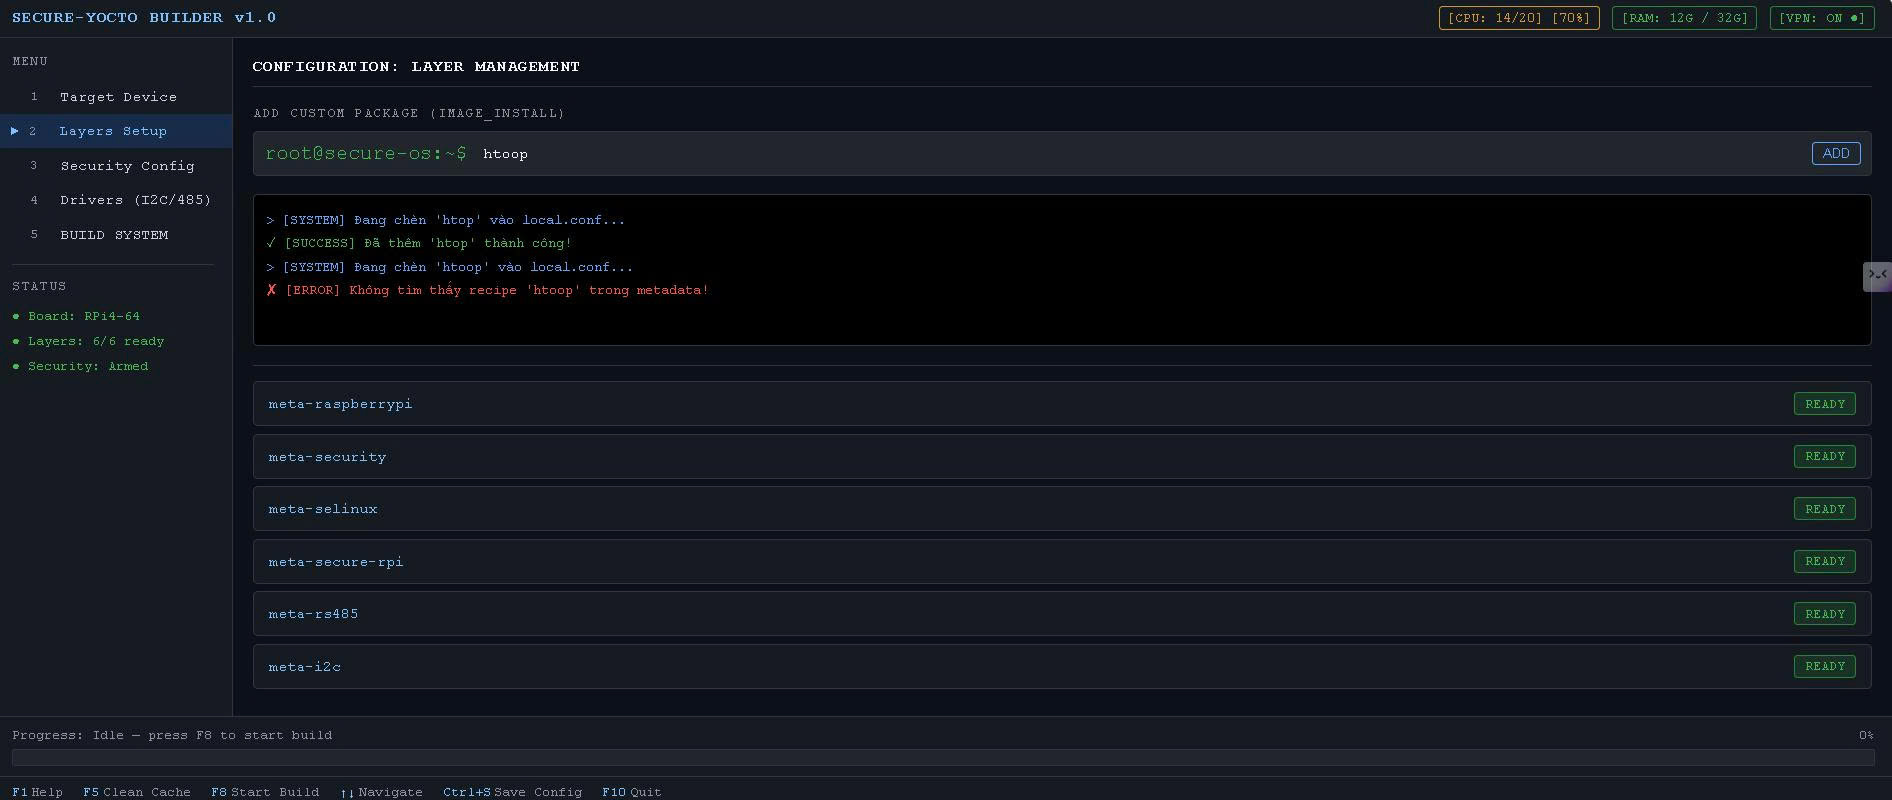
\includegraphics[width=\textwidth]{image/image_be4272.jpg}
    \end{minipage}
    \caption{Kết quả kiểm tra và thêm gói phần mềm thủ công.}
    \label{fig:package-management}
\end{figure}

\subsubsection{Cấu hình bảo mật hệ thống (Security Hardening)}

Giao diện cung cấp các checkbox để bật/tắt các tính năng bảo mật cốt lõi như SELinux, dm-verity, Read-only RootFS và mã hóa tệp tin. Mỗi thao tác đều được Backend xử lý thông qua biểu thức chính quy (Regex) để comment hoặc uncomment các dòng cấu hình tương ứng.

\begin{figure}[H]
    \centering
    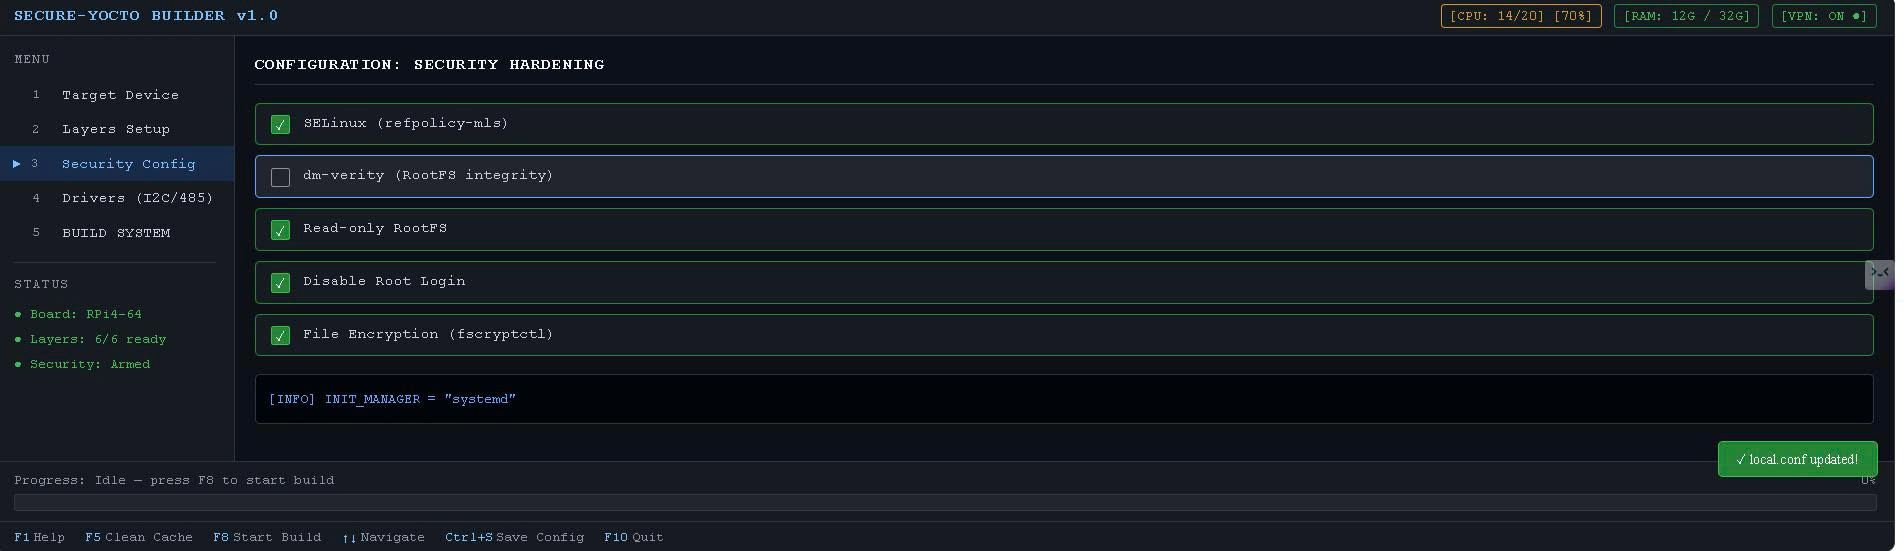
\includegraphics[width=0.85\textwidth]{image/image_be425a.jpg}
    \caption{Bảng điều khiển các tính năng bảo mật nâng cao.}
    \label{fig:security-hardening-ui}
\end{figure}

\subsubsection{Quản lý Driver ngoại vi (Peripheral Drivers)}

Người dùng có thể kích hoạt nhanh các giao tiếp phần cứng như RS-485 hoặc I\textsuperscript{2}C thông qua việc nạp các Device Tree Overlay và Kernel Module tương ứng.

\begin{figure}[H]
    \centering
    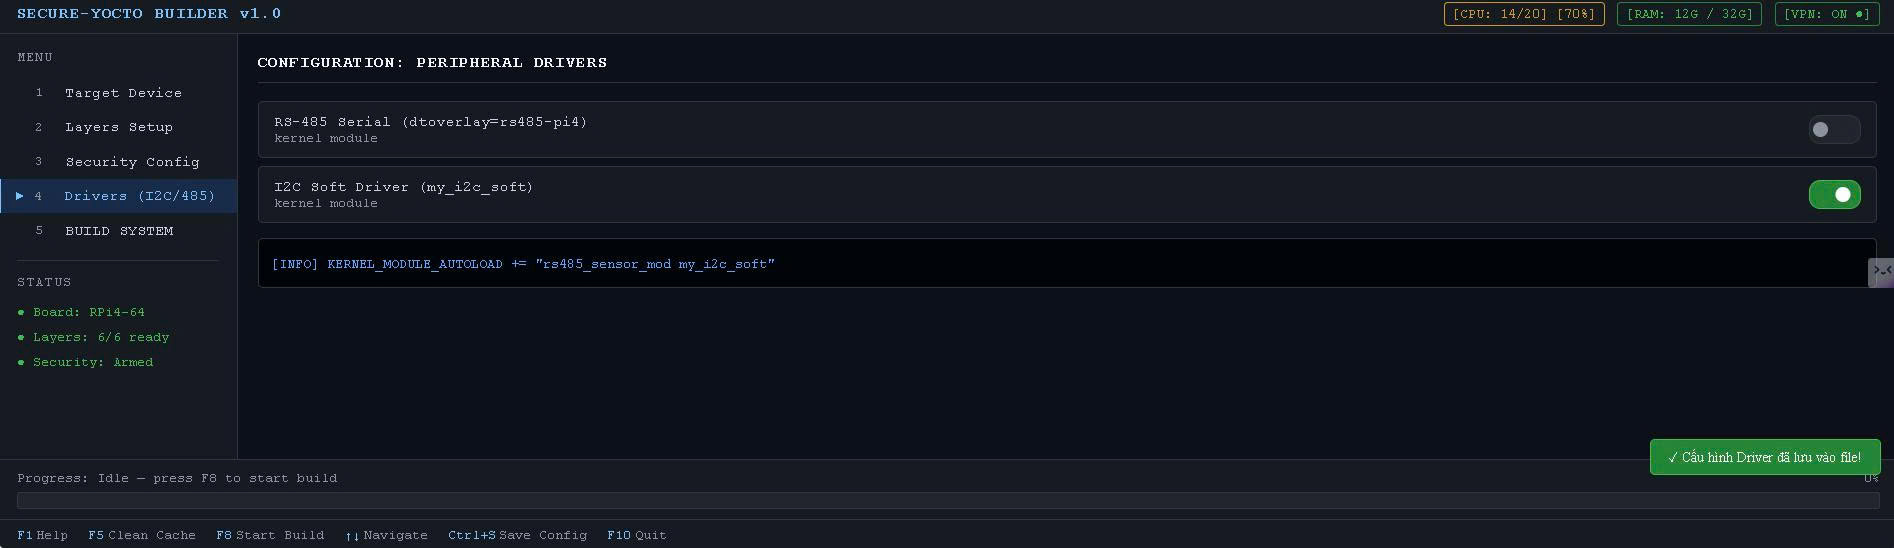
\includegraphics[width=0.85\textwidth]{image/image_be4254.jpg}
    \caption{Giao diện bật/tắt Driver RS-485 và I\textsuperscript{2}C Soft Driver.}
    \label{fig:driver-management-ui}
\end{figure}

\subsubsection{Hệ thống Build và Giám sát tiến độ}

Giao diện Build System hiển thị bảng tóm tắt cấu hình trước khi bắt đầu. Trong quá trình thực thi lệnh \texttt{bitbake}, thanh tiến độ (\textit{Progress Bar}) được cập nhật liên tục dựa trên các tác vụ thực tế đang chạy.

\begin{figure}[H]
    \centering
    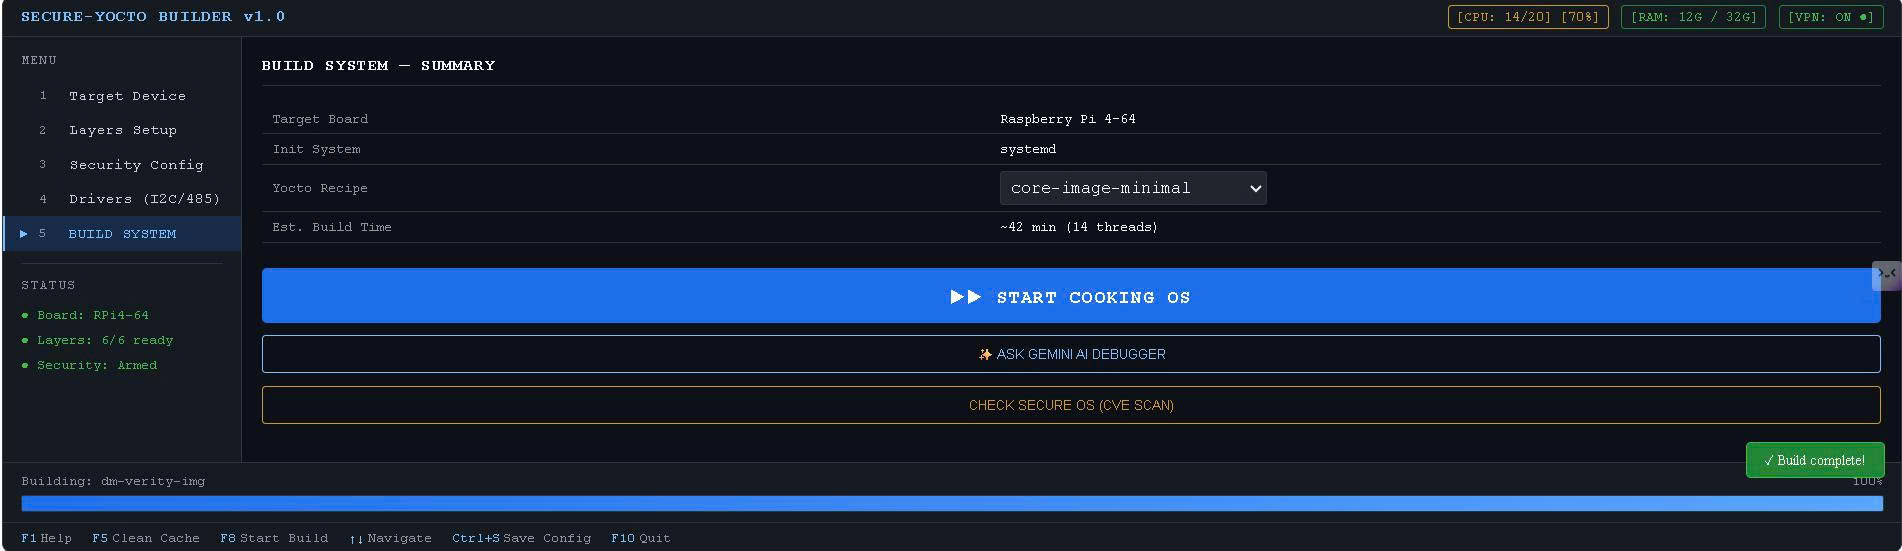
\includegraphics[width=0.85\textwidth]{image/image_be4252.jpg}
    \caption{Tổng kết cấu hình và thanh tiến độ hoàn thành bản build.}
    \label{fig:build-progress-ui}
\end{figure}

\subsubsection{Tính năng thông minh: AI Debug và CVE Scan}

Đây là hai tính năng nổi bật của công cụ:

\begin{itemize}
    \item \textbf{AI Diagnosis:} Tích hợp Gemini AI để giải thích các lỗi cú pháp phức tạp trong Yocto (ví dụ: lỗi trong tệp \texttt{bblayers.conf}) và đưa ra giải pháp khắc phục bằng tiếng Việt.
    \item \textbf{CVE Scan:} Hiển thị danh sách các lỗ hổng bảo mật được phát hiện trong Image, phân loại theo mức độ từ Trung bình đến Nghiêm trọng (\textit{Critical}).
\end{itemize}

\begin{figure}[H]
    \centering
    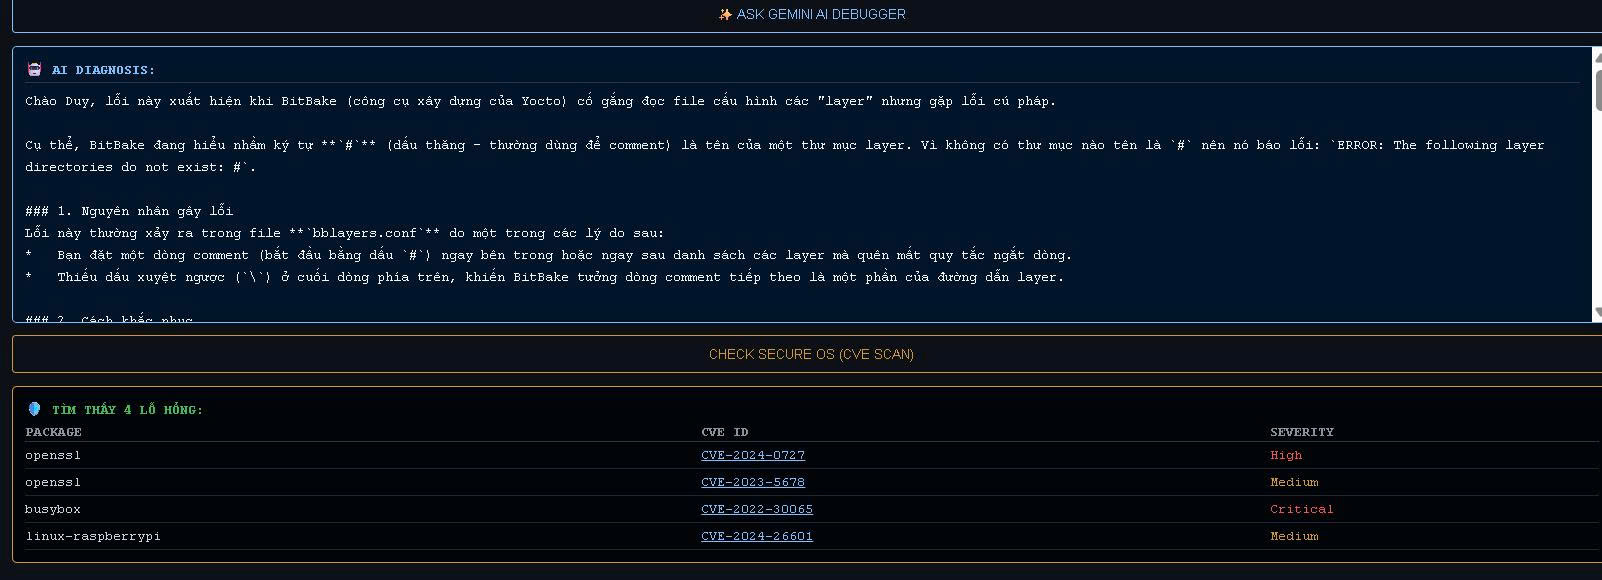
\includegraphics[width=0.85\textwidth]{image/image_be423a.jpg}
    \caption{Kết quả phân tích lỗi của AI và bảng danh sách lỗ hổng CVE.}
    \label{fig:ai-debug-cve-scan}
\end{figure}

\subsection{Đánh giá và nhận xét}

Dựa trên kết quả thực nghiệm, công cụ Secure-Yocto Builder đạt được các tiêu chí sau:

\subsubsection{Về tính năng và vận hành}

\begin{itemize}
    \item \textbf{Độ chính xác:} Các thao tác cấu hình thông qua giao diện Web được phản ánh chính xác vào các tệp hệ thống như \texttt{local.conf} và \texttt{bblayers.conf}, giúp loại bỏ lỗi cú pháp do người dùng chỉnh sửa thủ công.
    \item \textbf{Tính hiệu quả:} Việc tích hợp AI Debugger giúp giảm đáng kể thời gian tìm kiếm lỗi trên các diễn đàn kỹ thuật; các lỗi liên quan đến Layer hoặc cú pháp BitBake được giải thích rõ ràng và kèm hướng dẫn khắc phục cụ thể.
    \item \textbf{An toàn:} Module CVE Scan giúp lập trình viên nhận diện sớm các gói phần mềm lỗi thời, từ đó có phương án cập nhật hoặc vá lỗi trước khi triển khai thiết bị.
\end{itemize}

\subsubsection{Về trải nghiệm người dùng (UX)}

\begin{itemize}
    \item Giao diện TUI mang lại trải nghiệm chuyên nghiệp, tốc độ phản hồi nhanh nhờ cơ chế xử lý bất đồng bộ (\texttt{fetch} và \texttt{async/await}).
    \item Hệ thống thông báo (\textit{Toast Message}) và vùng hiển thị nhật ký (\textit{Log Box}) cung cấp thông tin kịp thời về trạng thái của từng tác vụ cấu hình.
\end{itemize}

\subsubsection{Hạn chế còn tồn tại}

\begin{itemize}
    \item Tốc độ build vẫn phụ thuộc hoàn toàn vào tài nguyên phần cứng của máy chủ thực hiện build.
    \item Hiện tại hệ thống mới hỗ trợ một số nền tảng phổ biến như Raspberry Pi 4 và QEMU; cần mở rộng thêm cho các dòng SoC khác trong tương lai.
\end{itemize}

\section{Hệ thống OTA}

Sau khi hoàn tất quá trình tích hợp và cấu hình, hệ thống OTA đã được triển khai thực tế trên thiết bị Raspberry Pi 4. Kết quả cho thấy quy trình cập nhật hoạt động ổn định, đúng với thiết kế logic ban đầu.

\subsection{Giao diện quản trị Web (Web UI)}

Hệ thống sử dụng máy chủ Mongoose tích hợp sẵn trong SWUpdate để cung cấp giao diện cập nhật trực quan qua trình duyệt Web.

\begin{figure}[H]
    \centering
    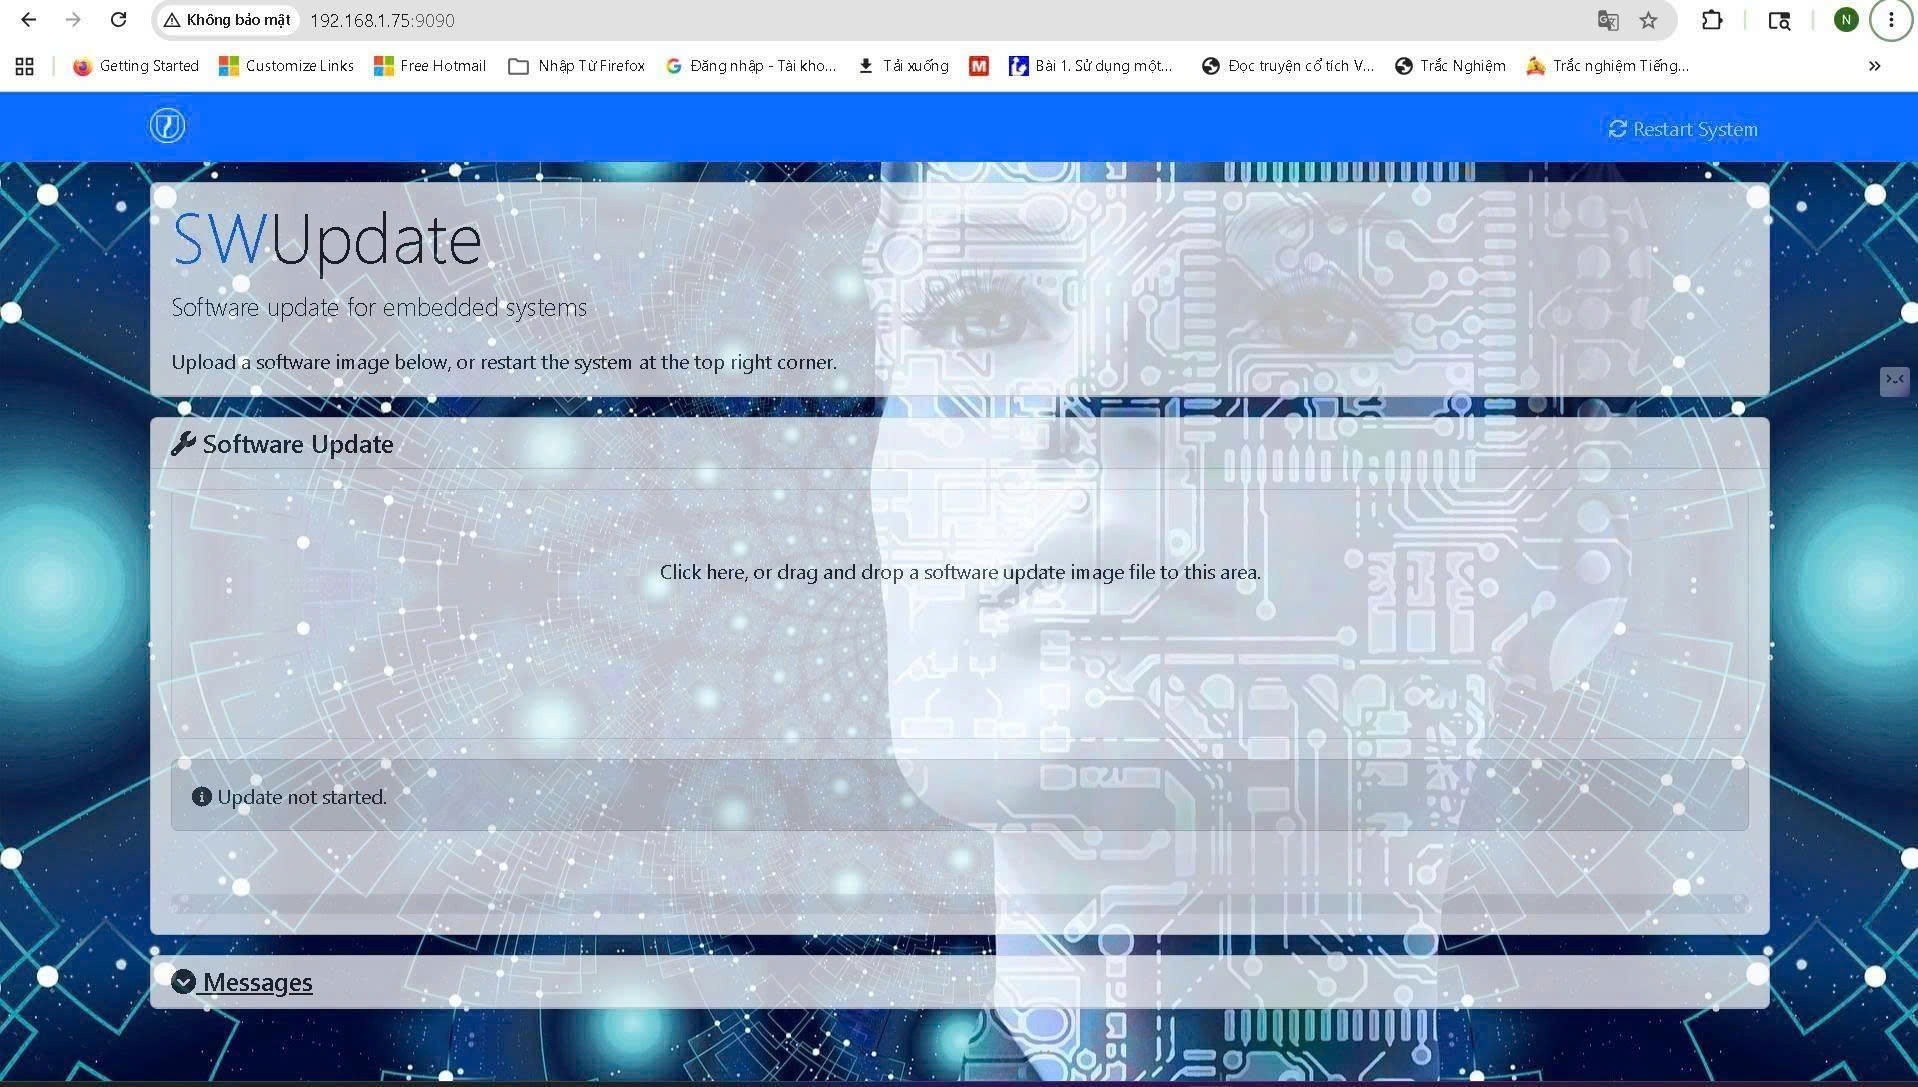
\includegraphics[width=0.85\textwidth]{image/mongo.jpg}
    \caption{Giao diện UI người dùng}
    \label{fig:build-progress-ui}
\end{figure}

\begin{itemize}
    \item \textbf{Truy cập:} Người dùng truy cập thông qua địa chỉ IP của thiết bị tại cổng 9090 (ví dụ: \texttt{http://192.168.1.75:9090}).

    \item \textbf{Chức năng:} Giao diện cho phép người dùng kéo-thả tập tin cập nhật có định dạng \texttt{.swu}. Hình ảnh thực tế (Hình~5.x) cho thấy giao diện Web UI hiển thị trạng thái sẵn sàng, cho phép quản lý việc tải lên Image mới một cách dễ dàng mà không cần can thiệp vào dòng lệnh.
\end{itemize}

\subsection{Quá trình thực thi và phân tích Log hệ thống}

Quá trình cập nhật được theo dõi trực tiếp thông qua Terminal của Raspberry Pi. Dựa trên kết quả thực thi (Hình~6.13), quy trình diễn ra qua các bước sau:

\begin{figure}[H]
    \centering
    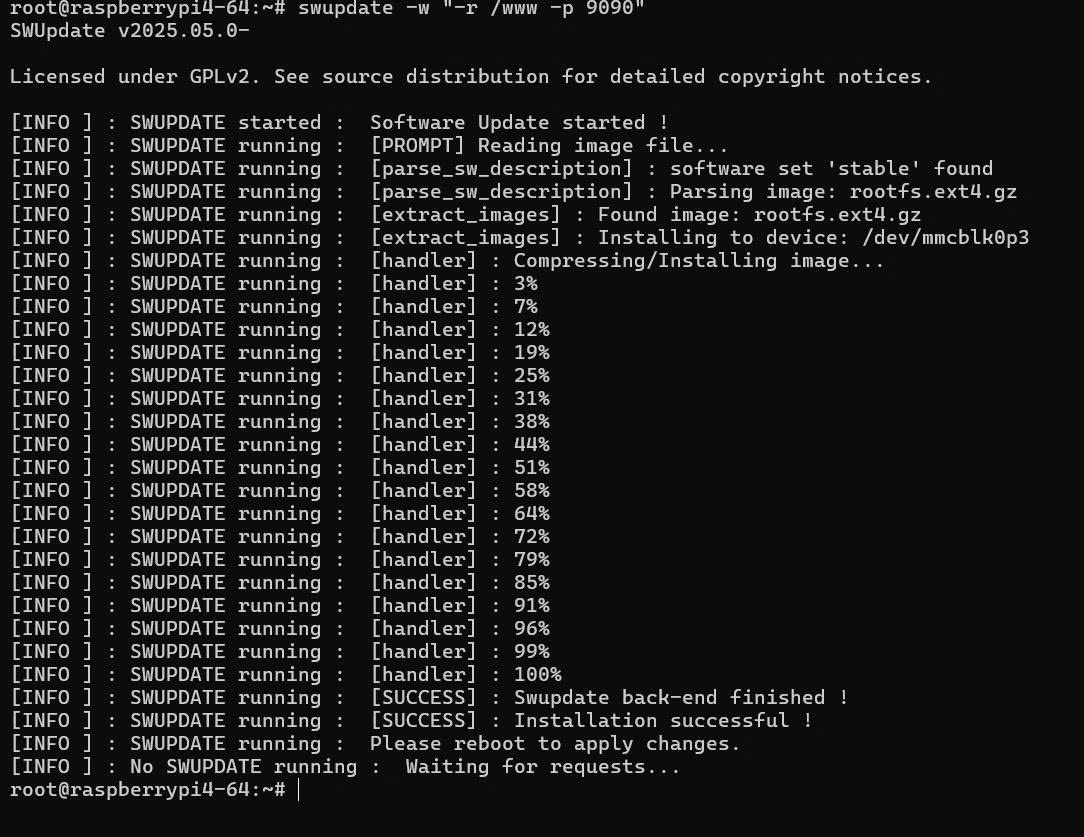
\includegraphics[width=0.85\textwidth]{image/hehe.jpg}
    \caption{Kết quả OTA}
    \label{fig:OTA-prges}
\end{figure}

\begin{itemize}
    \item \textbf{Khởi tạo:} Daemon \texttt{swupdate} được kích hoạt với tham số \texttt{-w} để mở tiến trình lắng nghe kết nối từ Web UI.

    \item \textbf{Phân tích gói dữ liệu (Parsing):} Sau khi tập tin \texttt{.swu} được tải lên, bộ phân tích cú pháp \texttt{libconfig} đã trích xuất thành công tệp \texttt{sw-description}, xác định được bộ phần mềm là \texttt{stable} và tập ảnh hệ thống là \texttt{rootfs.ext4.gz}.

    \item \textbf{Cài đặt (Installation):}
    \begin{itemize}
        \item Hệ thống xác định phân vùng đích là \texttt{/dev/mmcblk0p3} (đúng với thiết kế Slot B để đảm bảo an toàn cho Slot đang chạy).
        \item Tiến trình ghi dữ liệu thô (\textit{raw}) được thực hiện với thanh trạng thái tiến triển từ 0\% đến 100\%.
    \end{itemize}

    \item \textbf{Hoàn tất:} Log hệ thống hiển thị thông báo \texttt{[SUCCESS]: Installation successful!}. Điều này xác nhận việc ghi dữ liệu và kiểm tra tính toàn vẹn (\textit{Checksum}) đã hoàn tất thành công.
\end{itemize}

\subsection{Đánh giá hiệu năng và độ tin cậy}

Từ kết quả thực nghiệm, hệ thống OTA đạt được các tiêu chí đánh giá sau:

\begin{itemize}
    \item \textbf{Tính ổn định:} Quá trình cập nhật diễn ra mượt mà, không xảy ra hiện tượng treo hệ thống hay lỗi phân mảnh dữ liệu nhờ cơ chế ghi trực tiếp thông qua Handler của SWUpdate.

    \item \textbf{Tính an toàn (Atomic Update):} Việc ghi dữ liệu vào phân vùng dự phòng giúp hệ thống luôn duy trì một bản hệ điều hành ổn định. Nếu quá trình cập nhật bị gián đoạn (ví dụ mất điện đột ngột), Slot chính vẫn không bị ảnh hưởng.

    \item \textbf{Tính trực quan:} Sự kết hợp giữa Web UI và Log Terminal giúp người quản trị dễ dàng theo dõi trạng thái cập nhật theo thời gian thực.

    \item \textbf{Thời gian đáp ứng:} Tốc độ giải nén và ghi dữ liệu phụ thuộc vào hiệu năng của thẻ nhớ SD hoặc eMMC trên Raspberry Pi, nhưng nhìn chung đáp ứng tốt yêu cầu cập nhật phần mềm từ xa trong môi trường công nghiệp.
\end{itemize}

\section{Dashboard giám sát}
\subsection{Thiết kế giao diện Dashboard CoreIot}
Giao diện giám sát và điều khiển (Dashboard) đóng vai trò là lớp ứng dụng trong mô hình IoT, là cầu nối trực tiếp giữa dữ liệu kỹ thuật và người sử dụng. Trong đồ án này, Dashboard được xây dựng với mục tiêu tối ưu hóa khả năng quan sát tập trung và phản hồi nhanh chóng trước các sự cố môi trường tại nhà kho.

\begin{figure}[H]
    \centering
    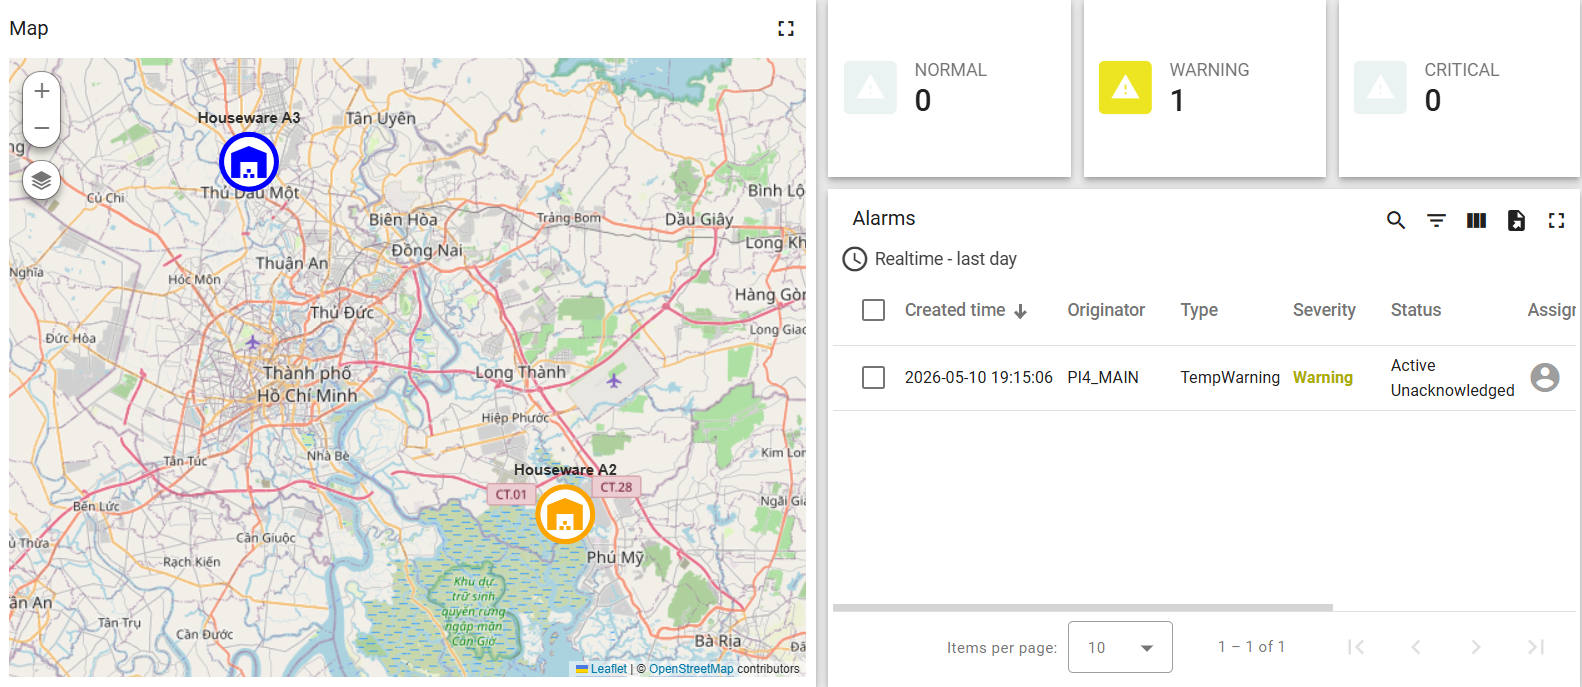
\includegraphics[width=1\linewidth]{image/coreiotdb.png}
    \caption{Trang chủ Dashboard CoreIot}
    \label{fig:placeholder}
\end{figure}

Tại giao diện chính, hệ thống tích hợp Widget Bản đồ (Map) dựa trên nền tảng OpenStreetMap, cho phép quản lý đa điểm các nhà kho phân tán tại các khu vực khác nhau (như TP. Hồ Chí Minh và Bình Dương). Để nâng cao tính trực quan, trạng thái của từng nhà kho được định nghĩa qua các màu sắc đặc trưng của biểu tượng (Marker):
\begin{itemize}
  \item \textbf{Màu xanh dương:} Phản ánh tình trạng Gateway mất kết nối với máy chủ Cloud, giúp kỹ thuật viên phát hiện ngay lập tức các sự cố về hạ tầng mạng.

  \item \textbf{Màu xanh lá:} Xác nhận hệ thống đang vận hành ổn định, mọi thông số môi trường đều nằm trong ngưỡng an toàn cho phép.

  \item \textbf{Màu cam (Warning) \& Màu đỏ (Critical):} Hệ thống sẽ tự động chuyển đổi sang các màu sắc này khi dữ liệu cảm biến vượt ngưỡng cài đặt hoặc có sự cố cháy nổ, xâm nhập.
\end{itemize}

\begin{figure}[H]
    \centering
    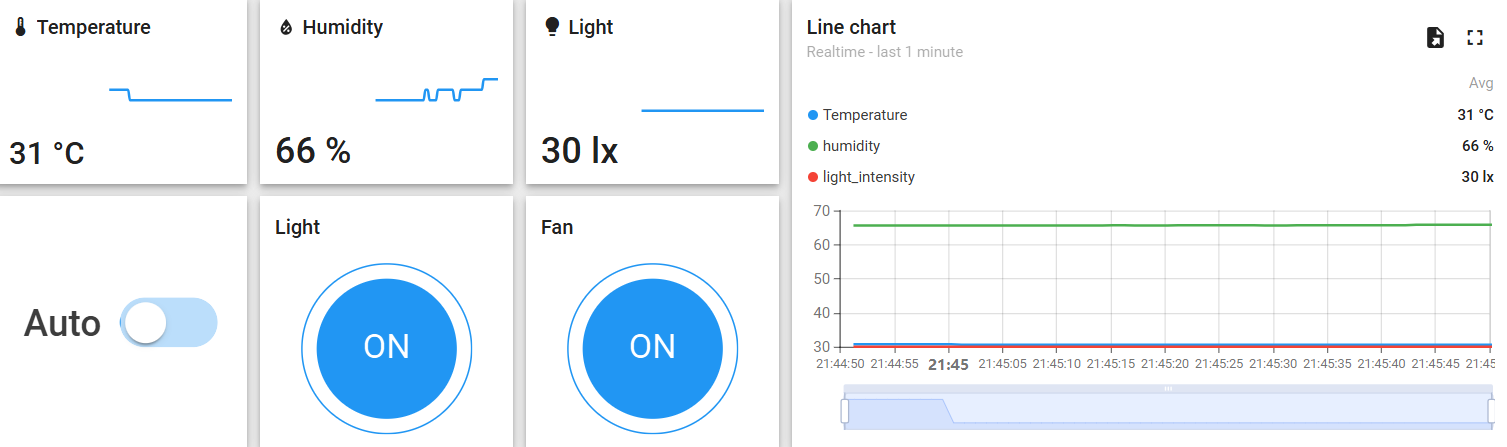
\includegraphics[width=1\linewidth]{image/coreiotdb2.png}
    \caption{Trang thiết bị Dashboard CoreIot}
    \label{fig:placeholder}
\end{figure}

Khi người dùng truy cập vào một nhà kho cụ thể, giao diện sẽ hiển thị chi tiết các thông số kỹ thuật nội khu. Các dữ liệu về Nhiệt độ, Độ ẩm và Cường độ ánh sáng không chỉ được hiển thị dưới dạng số thực thời gian thực mà còn được trực quan hóa bằng biểu đồ đường. Việc sử dụng biểu đồ thời gian thực với chu kỳ cập nhật liên tục giúp người vận hành phân tích được xu hướng biến thiên của môi trường, từ đó đưa ra các dự báo sớm về tình trạng hư hỏng hàng hóa hoặc lãng phí điện năng.

Kết hợp linh hoạt giữa cơ chế Tự động hóa  và quyền Can thiệp thủ công, tạo nên một quy trình vận hành khép kín và an toàn. Với chế độ "Auto", người dùng kích hoạt hệ thống xử lý thông minh; tại đây, các thiết bị chấp hành như đèn và quạt sẽ tự động phản hồi dựa trên dữ liệu từ cảm biến, chẳng hạn như tự động bật đèn khi cường độ ánh sáng xuống dưới 100 lx hoặc kích hoạt hệ thống làm mát khi nhiệt độ tăng cao vượt ngưỡng. Nhằm đảm bảo tính kiểm soát trong các tình huống bảo trì hoặc khẩn cấp, hệ thống cho phép tắt chế độ Auto để chuyển sang cơ chế điều khiển thủ công, giúp người dùng trực tiếp thao tác qua các nút nhấn cảm ứng trên giao diện. Đặc biệt, trạng thái phản hồi từ thiết bị được hiển thị trực quan qua hiệu ứng ánh sáng trên Dashboard, đảm bảo tính xác thực tuyệt đối giữa lệnh điều khiển trên phần mềm và trạng thái hoạt động thực tế của phần cứng tại nhà kho.

\subsection{Thiết kế giao diện HDMI Dashboard}

Giao diện HDMI Dashboard được xây dựng nhằm trực quan hóa dữ liệu thu thập từ hệ thống nhúng và cung cấp công cụ giám sát trạng thái thiết bị theo thời gian thực. Toàn bộ giao diện được phát triển trên nền tảng Python kết hợp với thư viện PyQt5, một lựa chọn phù hợp cho ứng dụng desktop nhờ khả năng xử lý sự kiện tốt, mô hình lập trình hướng đối tượng chặt chẽ và cơ chế signal–slot hỗ trợ cập nhật dữ liệu động mà không cần làm mới toàn bộ cửa sổ. Các dữ liệu từ hệ thống backend được truyền về dashboard và hiển thị liên tục theo chu kỳ, đảm bảo tính thời gian thực trong quá trình giám sát.

Về mặt cấu trúc, HDMI Dashboard được tổ chức thành nhiều module chức năng nhằm đảm bảo tính rõ ràng và dễ bảo trì. Các thành phần chính bao gồm lớp giao diện chính (Main Window), module hiển thị dữ liệu cảm biến, module cảnh báo hệ thống và module xử lý kết nối dữ liệu. Mỗi module đảm nhiệm một vai trò riêng biệt, trong đó lớp giao diện chính đóng vai trò điều phối và quản lý toàn bộ luồng hiển thị. Dựa trên các ảnh chụp màn hình thực tế, có thể thấy giao diện được chia thành ba khu vực chính: thanh điều hướng (Dashboard, Sensors, Notifications), khu vực hiển thị thông số chính và khu vực điều khiển.

Hình ảnh tổng thể của dashboard được trình bày trong Hình~\ref{fig:HDMI_dashboard}. Tại đây, các thông số môi trường quan trọng như nhiệt độ (29.00°C), độ ẩm (58.51\%) và nồng độ bụi mịn PM2.5 (12.16 µg/m³) được hiển thị nổi bật dưới dạng các ô thông tin riêng biệt. Bên cạnh đó, khu vực camera được tích hợp nhằm cung cấp luồng hình ảnh trực tiếp từ không gian giám sát. Khu vực Notifications hiển thị danh sách các cảnh báo với số lượng (20) và nút “View All” để xem chi tiết. Phía dưới cùng là bảng điều khiển (Controls) chứa ba nút chức năng (BUTTON 1, BUTTON 2, BUTTON 3), cho phép người dùng tương tác trực tiếp với hệ thống nhúng qua giao diện.

\begin{figure}[H]
    \centering
    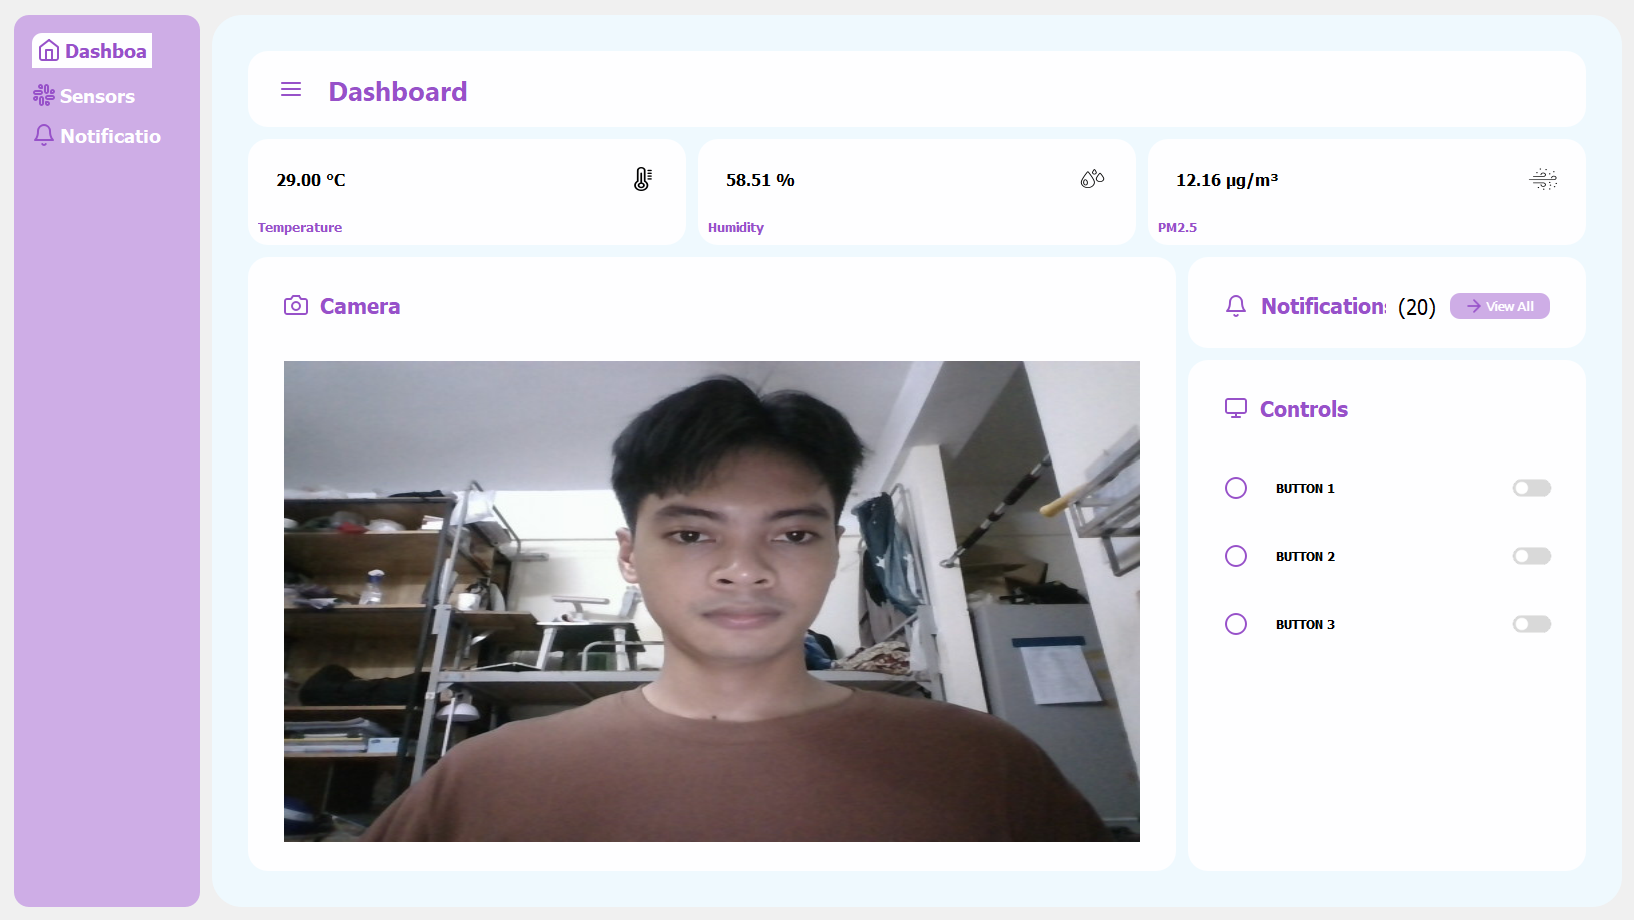
\includegraphics[width=1\linewidth]{image/dbdg2.png}
    \caption{Giao diện HDMI Dashboard tổng thể}
    \label{fig:HDMI_dashboard}
\end{figure}

Ngoài giao diện chính, hệ thống còn cung cấp hai màn hình chức năng riêng biệt cho việc xem dữ liệu cảm biến chi tiết và quản lý thông báo. Hình ảnh từ màn hình Sensors (Hình~\ref{fig:sensors_view}) cho thấy dữ liệu được trình bày dưới dạng bảng cho từng cảm biến. Ví dụ, Sensor 1 hiển thị các cột gồm nhiệt độ (Temp), độ ẩm (Humid), PM2.5 và thời gian (Time) với các giá trị cụ thể (60, 20, 1.5, 11:15 AM 02-12-2025). Màn hình này cho phép theo dõi lịch sử dữ liệu theo từng mốc thời gian, hỗ trợ đối chiếu và phân tích xu hướng biến đổi của các chỉ số môi trường.

\begin{figure}[H]
    \centering
    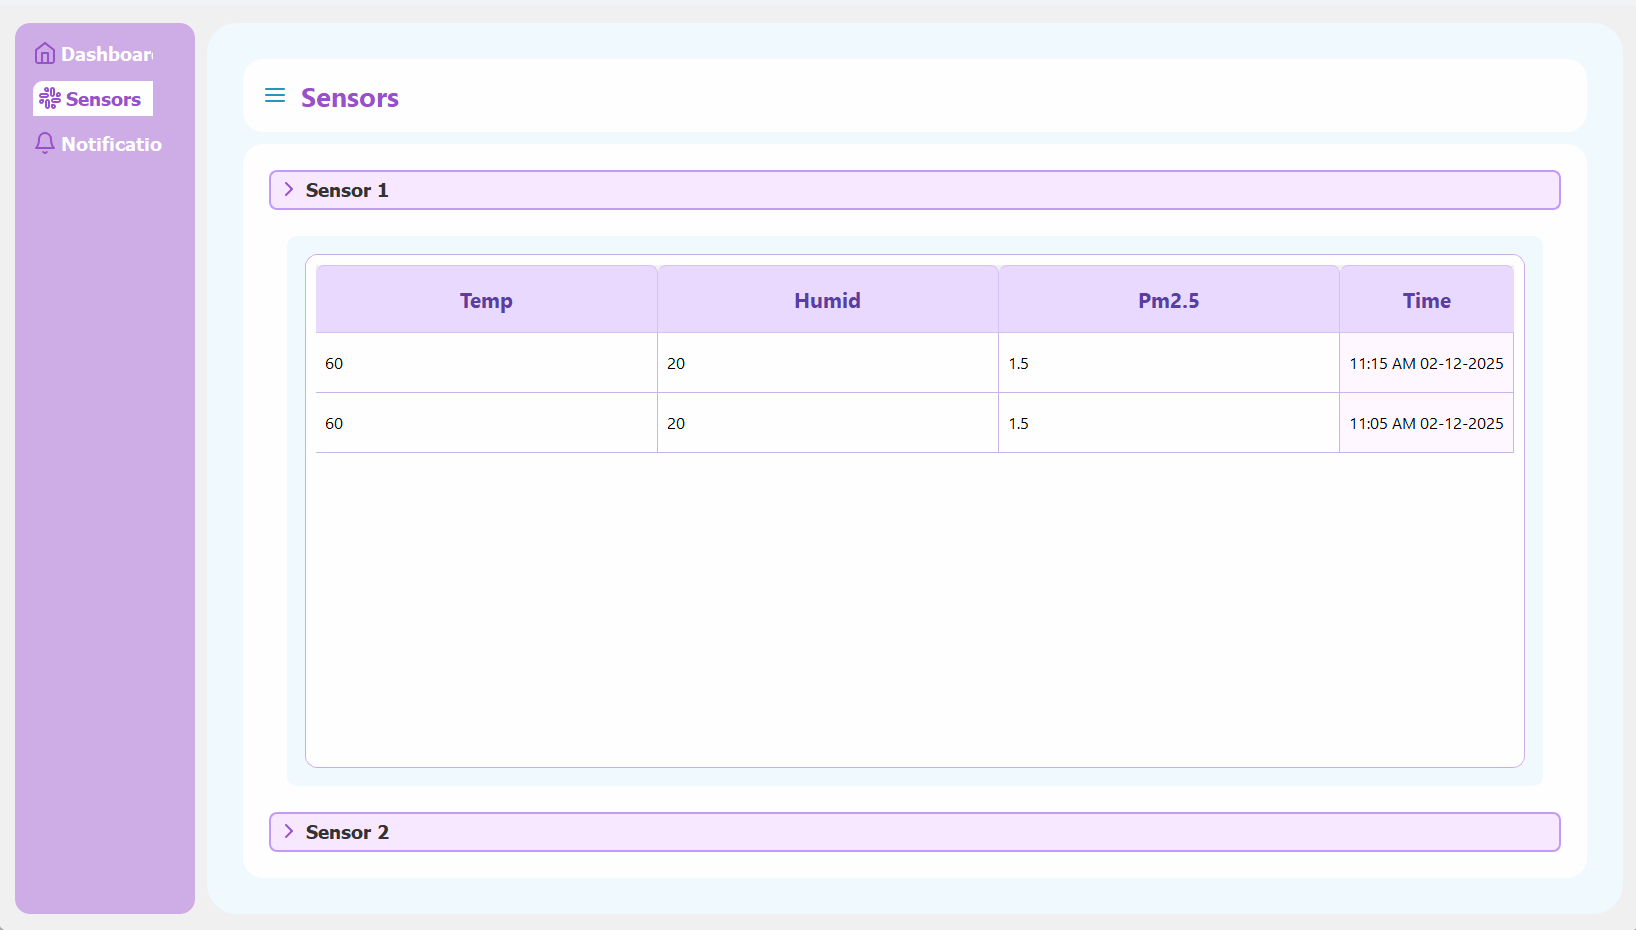
\includegraphics[width=0.8\linewidth]{image/dbsensor.png}
    \caption{Màn hình hiển thị dữ liệu các cảm biến}
    \label{fig:sensors_view}
\end{figure}

Màn hình Notifications (Hình~\ref{fig:notifications_view}) tập trung vào các thông báo hệ thống, được thiết kế dưới dạng danh sách hoặc các khối tin nhắn cảnh báo. Giao diện này giúp người quản trị nhanh chóng nắm bắt các sự kiện bất thường như vượt ngưỡng nhiệt độ, độ ẩm, hoặc PM2.5. Mặc dù hình ảnh chỉ hiển thị các tab điều hướng, nhưng trong quá trình hiện thực, module Notifications đã được tích hợp cơ chế lưu trữ và phân loại thông báo theo mức độ ưu tiên.

\begin{figure}[H]
    \centering
    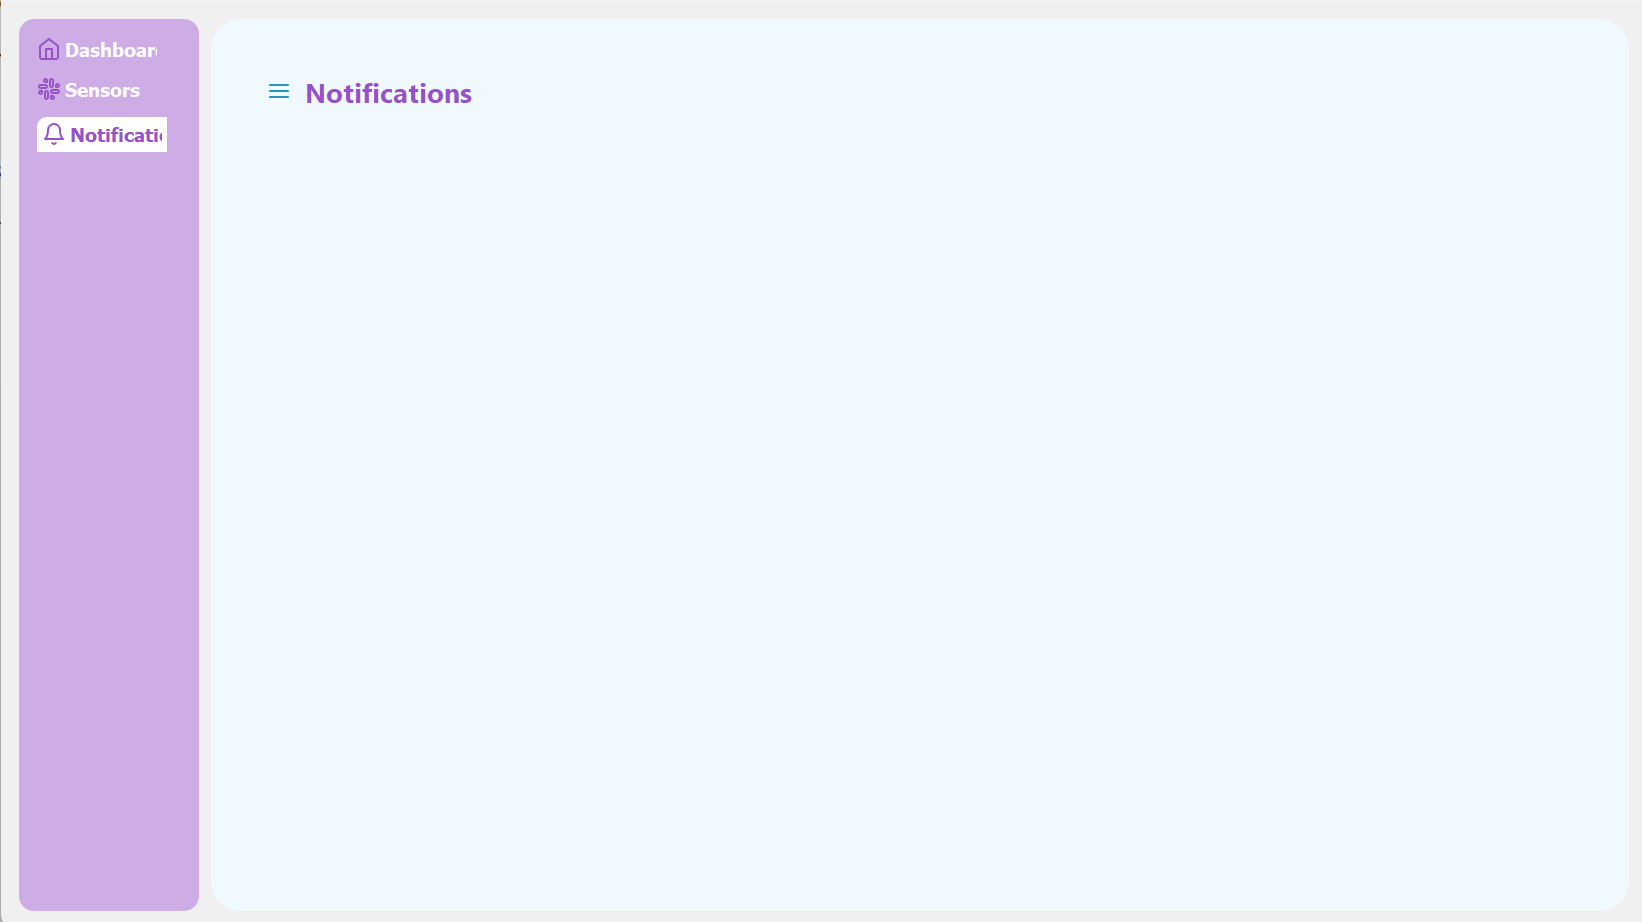
\includegraphics[width=0.8\linewidth]{image/dbnoti.png}
    \caption{Giao diện tab Notifications}
    \label{fig:notifications_view}
\end{figure}

Vận hành tổng thể của dashboard dựa trên cơ chế nhận dữ liệu định kỳ từ backend. Mỗi khi có dữ liệu mới (nhiệt độ, độ ẩm, PM2.5, trạng thái cảm biến), hệ thống sẽ phát tín hiệu (signal) qua kết nối MQTT hoặc HTTP, và dashboard bắt tín hiệu đó để cập nhật trực tiếp lên các widget tương ứng mà không cần tải lại toàn bộ giao diện. Các nút điều khiển (BUTTON 1–3) được gắn kết với các lệnh điều khiển thiết bị (ví dụ bật/tắt quạt, relay, thay đổi chế độ hoạt động) thông qua cơ chế gọi hàm callback. Nhờ vậy, người dùng vừa có thể giám sát thông số, vừa có thể can thiệp từ xa ngay trên dashboard.

Nhìn chung, việc sử dụng PyQt5 kết hợp với kiến trúc module hóa và phân chia rõ ràng các màn hình chức năng đã giúp HDMI Dashboard đạt được sự cân bằng giữa tính linh hoạt trong phát triển, khả năng mở rộng trong tương lai, và đáp ứng yêu cầu giám sát hệ thống nhúng theo thời gian thực.
